
\chapter{自动语音识别及序列建模综述}
\label{chap:intro}

自动语音识别技术(Automatic Speech Recognition)是一种将人的语音转换为文本的技术,
序列建模则是该技术不同于传统模式分类技术的核心。
%
本章中我们会最先介绍自动语音识别的框架,并概述每个子模块的基本设计。
近年来,深度学习模型被引入到语音识别的声学和语言建模当中替代传统分类器(NN-HMM),显著改善了模式分类问题的精度,从而改善了语音识别的准确度~\cite{CD-DNN-HMM-dahl2012,DNN4ASR-hinton2012}。 另一方面,语音识别本质上是一个序列标注问题。NN-HMM模型的序列关联性依赖于隐马尔科夫模型进行建模,而隐马尔科夫模型的状态转移建模能力有限。除此之外,NN-HMM模型对深度学习模型和隐马尔科夫模型进行分别训练,缺少了整体优化也将影响最终的模式分类性能。因此我们着重介绍了深度学习背景下的序列建模研究。
在最后一部分,得益于分类能力有所提升,深度学习模型时序建模能力被用于搭建端到端语音识别系统。其得益于更好的序列分类能力和更简单推理搜索框架,已经成为当前研究的热点。


\section{自动语音识别框架}
\label{chap:intro-asr}

这一章我们将主要介绍在大词汇连续语音识别中一些基本内容,图~\ref{fig:asr}中所描绘的几个部分都会在本章描述。这主要包括:特征提取前端、子词单元的挑选、隐马尔科夫、解码搜索、语言模型等内容。

\subsection{特征提取}
\label{sec:feat_extra}
语音信号原始形态是一种连续的波形语音,为了能进行 更有效的识别,通常我们会先将连续的波形转换为一个离散的实数序列向量$\mathbf{O}=\left[ \mathbf{o}_1, ..., \mathbf{o}_T \right]^\top$。每个向量是压缩语音变化的表示。这些矢量也称为特征矢量或观察特征矢量。语音信号是准静态信号,因此我们首先需要将其切割成多个重叠的离散段,通常是以10毫秒的间隔向后滑动25毫秒长的窗口。通过此方法提取的段称为帧。汉明窗口或汉宁窗口通常用于平滑,以减少边界效应,然后使用快速傅立叶变换将其从时域特征变换到频域特征。在得到频域上的复数特征后,通过利用不同的后处理方法可以得到不同特征:典型的有感知线性预测系数(Perceptual Linear Prediction, PLP)~\cite{hermansky1990perceptual}和梅尔倒谱系数(Mel-Frequency Cepstral Coefficients, MFCC)~\cite{davis1980comparison}。近来,由于深度神经网络拥有更强大的建模能力,研究者发现保留梅尔滤波器输出中维度之间的相关性的滤波器组特征(Filter Bank Feature, FBANK)~\cite{seide2011feature}更适合于深度神经网络利用,接下来将对这三种特征进行详细介绍:
\begin{itemize}
    \item 滤波器组特征 \\
    1. 在获得频谱的复杂特征之后,通常丢弃相位信息,并且仅留下复杂特征的幅度部分。然后通过梅尔频率缩放公式调整频率轴。最后,我们可以得到一个缩放的幅度频域特征:
    \begin{equation}
        \text{Mel}(f)=2595 \log_{10}(1+\frac{f}{500}) 
    \end{equation}
    2. 接下来,不同的滤波器包含不同的滤波器增益,并且将使用一组三角滤波器来对该频域特征进行下采样。最后,一个滤波器的输出是幅度特性滤波器中相应频率增益的自然对数乘积之和。通常,36组滤波器用于8K采样率,40组用于16K语音。
    \item 梅尔倒谱系数 \\
    梅尔倒谱系数特征在FBANK特征基础上去进一步利用离散余弦变换来计算倒谱系数以便减少滤波器的组之间相关性。通常是利用12个的倒谱系数加上归一化的功率自然对数组成一个13维的向量特征。
    \item 感知线性预测系数 \\
    1. 感知线性预测系数是另外一个倒谱的特征,它利用Bark公式来去缩放频率的轴:
    \begin{equation}
        \text{Bark}(f)=6\log \left( \left( \frac{f}{600}+1 \right)^{0.5}+\frac{f}{600} \right)
    \end{equation}
    2. 接着它利用功率谱(幅度的平方)来提取感知线性的识别特征,之后该功率谱会与一个临界的频带滤波器进行卷积操作并且通过等响度的曲线进行预加重操作。\\
    3. 最后通过利用线性预测分析来获得一种倒谱的系数。
\end{itemize}
在提取了原始声学的特征之后,通常会利用一些后处理方法:
\begin{itemize}
    \item 动态特征~\cite{furui1986speaker}:

    一阶动态特征的计算公式如下
    \begin{equation}
        \Delta_{\mathbf{o}_t}=\frac{\sum_{k=1}^K k(\mathbf{o}_{t+k}-\mathbf{o}_{t-k})}{2\sum_{k=1}^K{k^2}}
    \end{equation}
    其中$K$是动态特征计算窗的大小,通常设置为2。二阶动态特征是最为常用的,其计算方法和一阶一致,只不过将$\mathbf{o}_t$替换为$\Delta_{\mathbf{o}_t}$。在利用了动态特征后,特征的不同维度之间产生了相关性,这与后面一些声学模型建模方法中作出特征各维度之间独立性的假设产生了冲突。因此,为消除特征各维度之间不同的相关性,通常会利用线性投影的方法,如异方差线性判别分析(Heteroscedastic Linear Discriminant Analysis, HLDA)~\cite{kumar1998heteroscedastic}等。
    \item 特征正则化:

    特征正则化目标是消除声学特征中的非语音信号的变化,同时它也能将特征的值域范围进行归一化,这一操作对于深度神经网络来说特别重要。传统的正则化方法包括倒谱均值归一化(Cepstral mean normalisation, CMN)~\cite{atal1974effectiveness}, 倒谱方差归一化(Cepstral variance normalisation, CVN)\cite{woodland1995development}以及声道长度归一化(Vocal tract length normalisation, VTLN)~\cite{lee1996speaker}。其中倒谱均值归一化(CMN)将输入特征向量的每个维度的均值归一化为0,倒谱方差归一化(CVN)将输入特征向量的每个维度的方差归一化为1。归一化可以运用在不同层面-包括说话人层面及句子层面。声道长度归一化(VTLN)被用来减少声学特征中的说话人变化,它的原理是将来自于同一个说话人特征频率轴进行同样大小缩放。
\end{itemize}

\subsection{声学模型}
声学模型的作用是计算一个候选词序列$\mathbf{w}$生成出观测到的特征向量序列$\mathbf{O}$概率,即$p(\mathbf{O}|\mathbf{w})$。它从概率论角度提供了给定词标注之后语音信号的信号生成的过程。在传统GMM-HMM声学模型中,HMM建模了语音信号的序列性,GMM建模了特征向量生成的概率。在最新的基于深度神经网络的声学模型中,深度神经网络被用来计算特征向量生成概率。 GMM-HMM将在章节\ref{sec:hmm}中详细介绍,DNN-HMM将在章节\ref{sec:dnn_hmm}中详细介绍。声学模型是语音信号的识别系统中最核心部件之一,也是本论文研究重点。


\subsubsection{声学单元和参数绑定}
当进行小词汇语音信号的识别时,如识别数字时通常可以用隐马尔科夫模型直接建模独立的单词。然而当词汇数量从中等词汇上涨到大词汇(>10000)时,利用隐马尔科夫模型来建模每一个词汇变成了不可能事情。一个广泛利用的解决该问题方法为建模子词单元。

音素是一个被广泛利用的子词单元,它是语音信号的中最小声学元素。利用音素的好处是存在将每个词转换为音素标准,这样每个词能很容易的被分解成各个音素。在音素上建模的模型被称作音素模型,音素数目一般远远小于待识别词的个数。在当前最先进大词汇连续语音信号的识别系统 (Large Vocabulary Continuous Speech Recognition, LVCSR) 里,通常利用46个音素。

利用音素能更容易的获得足够数据以训练出更具有鲁棒性的模型参数。需要注意是当利用音素来建模时,需要提供一个字典用于将单词序列映射成子词单元序列,然后才能在子词单元的层面进行识别和运算。在识别最后,还需要将子词单元序列转换回单词序列。

目前有两种被广泛利用音素集合。一种是单音素,也称为上下文无关音素;另一种则是上下文相关音素。由于协同发音现象的影响,当前音素发音和前一个、后一个音素之间具有很强的相关性,所以在许多识别任务里,仅仅利用单音素效果不是很好。为了建模协同发音现象,目前最先进语音信号的识别系统利用的是上下文相关音素,其中三音速利用最为广泛,它将当前音素的前一个和后一个音素同时建模。

比如,以one来说,它对应三音素序列即扩展为one=\{sil−w−ah, w-ah-n, ah-n-sil\}。虽然利用更多的上下文信息可以建立更复杂的音素模型,如五音素~\cite{hain2005automatic}(quin-phones),但三音素依然是目前利用最广泛音素模型。根据是否考虑单词间的边界,三音素模型可以继续细分为跨单词三音素和单词内三音素。跨单词三音素允许三音素的扩展跨越单词:在两个单词边界,当前音素的前一个和后一个音素分别是上一个单词的最后一个音素和下一个单词第一个音素。词内三音素则相反,音素只能在单词的内部进行扩展。因此,在每个单词开头和结尾,是一个双音素。跨单词三音素在大规模词汇连续语音信号的识别系统里效果更好~\cite{woodland1994large}。

利用三音素后,声学单元个数将变得巨大。当利用46个单音素时,所有可能的三音素个数达到了$46^3=97336$,这一数字甚至超过了词表大小,不可能有充足数据能训练如此大的模型。目前一个通用解决该问题的方法是利用参数共享~\cite{young1993use, young1994tree}。它基本思想是将一些参数绑定在一起。参数共享可以存在于各个层面,包括音素,状态,高斯等。由于利用最广泛的是在状态共享层面,因而也被称为状态聚类。在利用状态聚类时,来自同一组的状态将共享状态输出分布,每一个实际状态输出分布被称为一个语素(senone),如图\ref{fig:state-tying}所示。
\begin{figure}[!htp]
  \centering
    \captionstyle{\centering}
    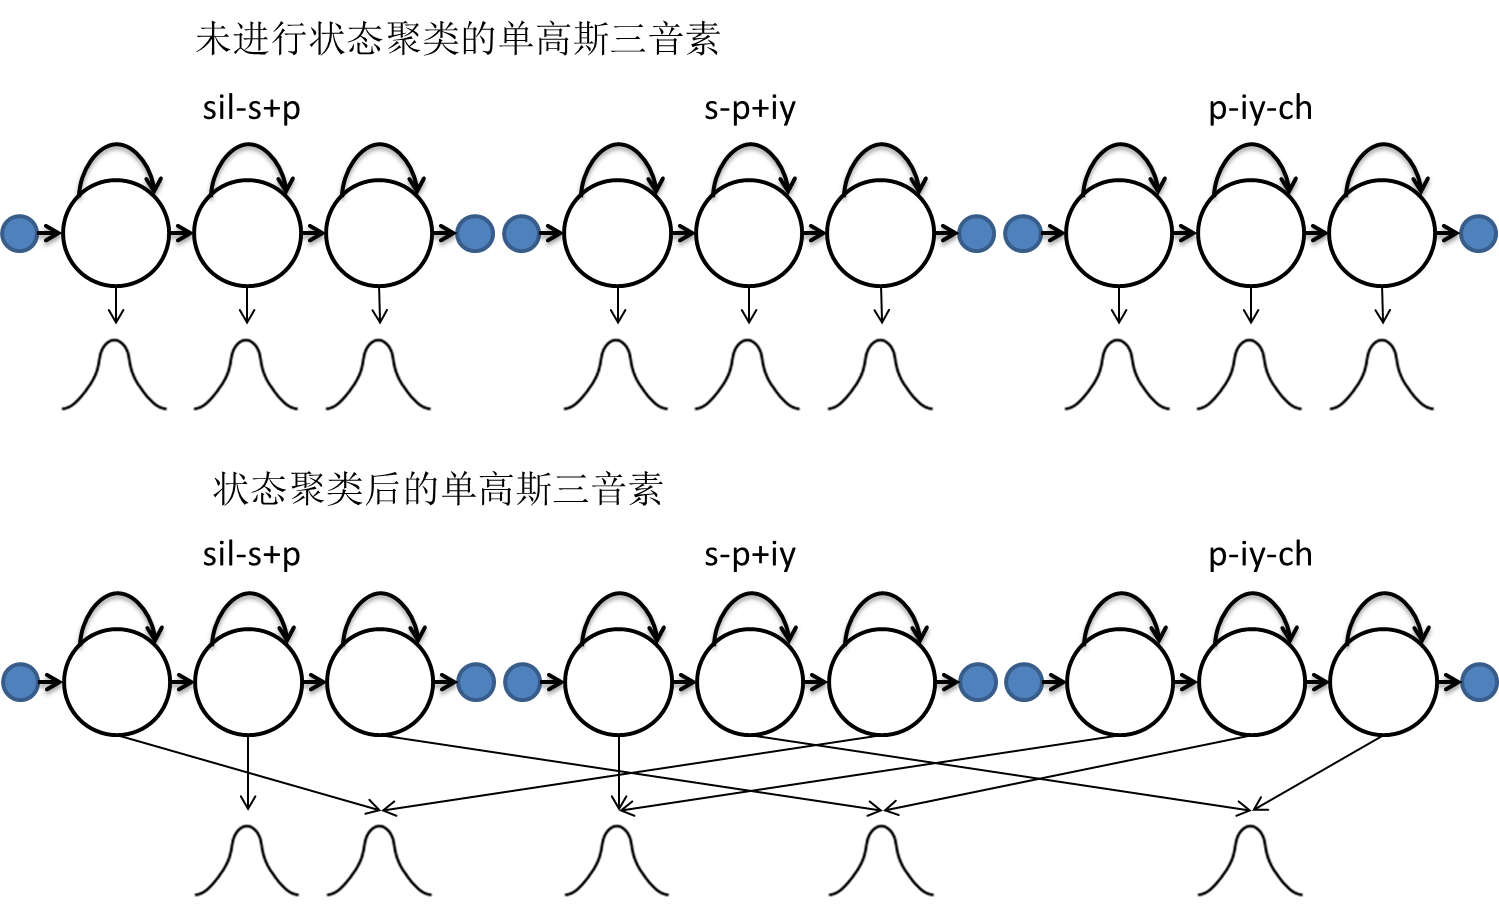
\includegraphics[width=.8\textwidth]{figure/state.png}
    \bicaption[fig:state-tying]{}{单高斯三音素的状态聚类}{Fig}{State clustering for single gaussian tri-phones}
\end{figure}

目前利用最广泛的聚类方法是基于数据驱动自底向上聚类。对训练集中存在的每一对语素之间计算一个距离,距离在某个阈值以内的语素将会被聚集在一起。数据驱动的主要问题在于当没有足够多训练数据时,这一方法将不再可靠,更严重的是,训练数据中不存在信息将无法被捕捉到。

另外一个更好的方法是利用音素决策树的方法来进行聚类。音素决策树是一棵包含了一系列关于每个音素左右上下文问题的二叉树,因为问题答案只有对和错。聚类自上而下开始,所有的状态都从根节点出发,通过回答上下文问题来分割左右儿子。直至处于当前节点的训练数据状态数目小于一个阈值,分割过程停止,此时叶子节点即为一个语素。决策树中的关键难题在于提问的顺序,目前最常用方法是在每次分裂时挑选能在分裂后似然增加的最大的那个问题。虽然这样决策树可能陷入局部最优,但它确实有效处理了对于不可见的三音素分类问题。

\subsubsection{隐马尔科夫模型 (HMM)}
\label{sec:hmm}
隐马尔科夫模型是一个统计学中的生成模型,在语音信号的识别领域获得了重大成功。在隐马尔科夫模型中,一个特定声学的单元,如一个单词或一个音素将被建模为一个有限状态机,而我们所观测到特征序列则是由该音频所对应的词序列连接成的有限状态机生成的。在每个时间单元,状态将以一个给定的概率分布发生转变:跳转到下一个状态或保持在当前状态。变换完成后,将由另一个概率函数生成一个特征向量。一个拥有三个输出状态的从左到右隐马尔科夫模型如图\ref{fig:hmm}所示,其中状态1和5是进入状态和退出状态,它们并不输出观测特征向量。这一结构是语音信号的识别中最常用的序列模型,我们将在第\ref{Sec:sgm-and-sdm}章节详细介绍这种结构,并将其与其他序列模型进行比较。

\begin{figure}[!htp]
  \centering
    \captionstyle{\centering}
    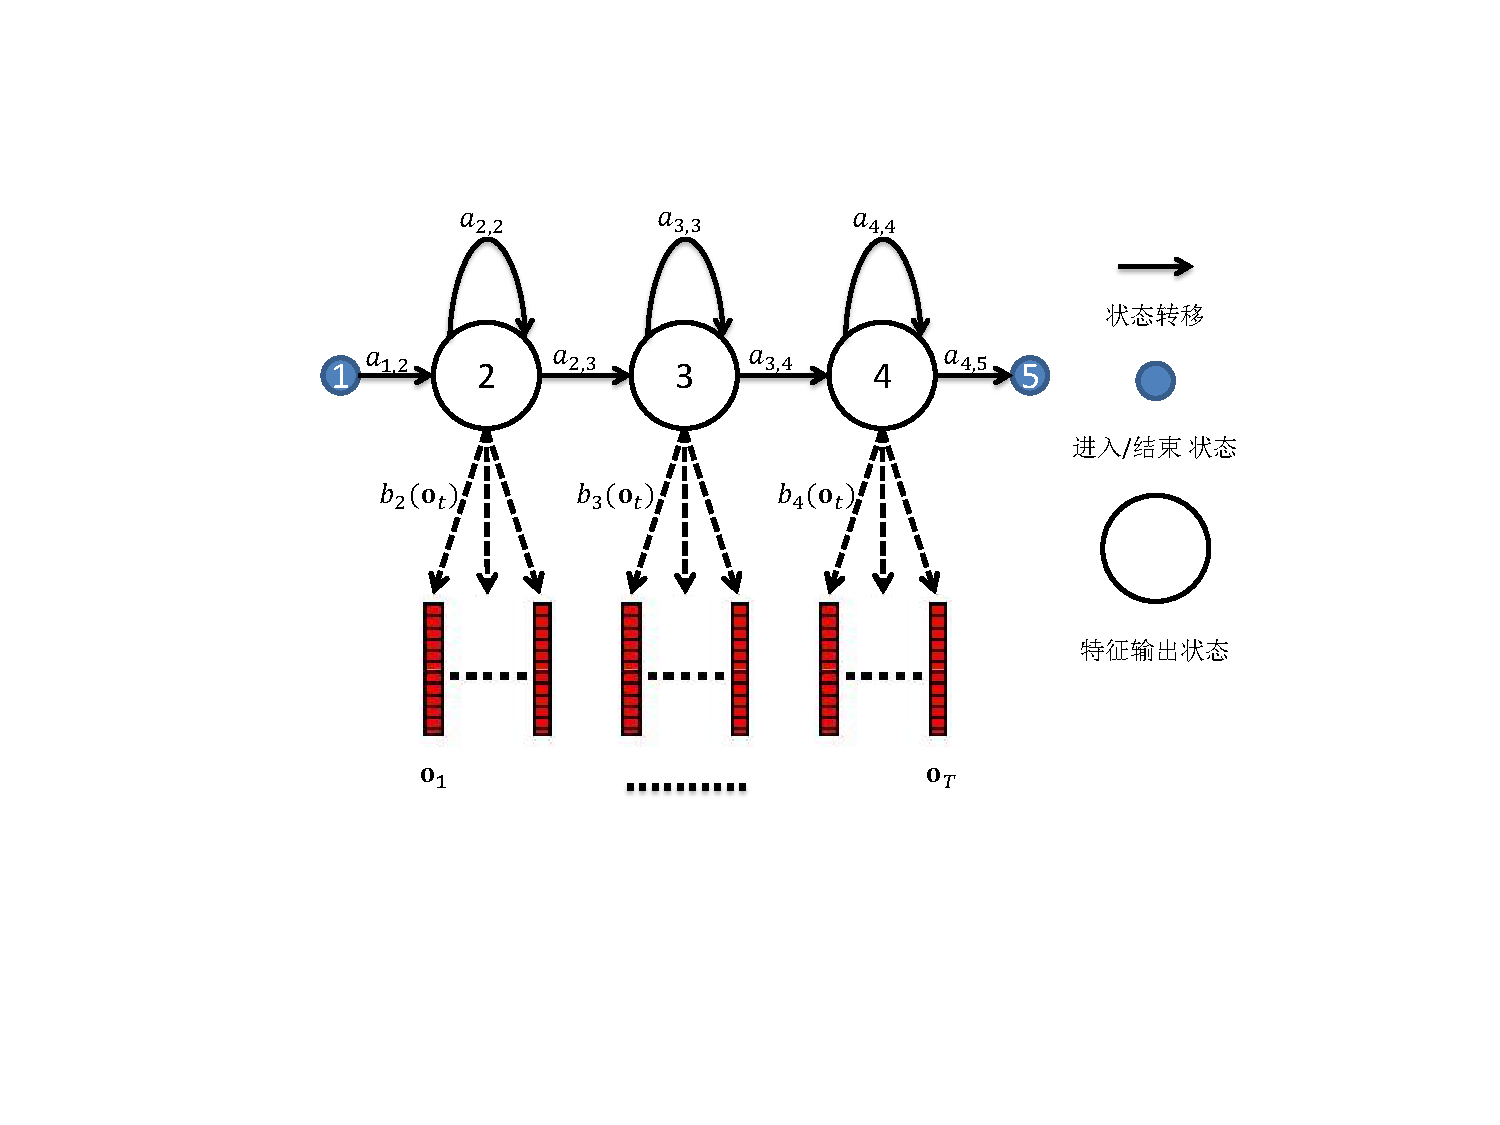
\includegraphics[trim = 3cm 5cm 4cm 3cm, clip=true, width=0.7\textwidth]{figure/hmm.pdf}
    \bicaption[fig:hmm]{}{隐马尔科夫模型}{Fig}{Hidden Markov Model}
\end{figure}

令$\mathbf{O}=[\mathbf{o}_1, ..., \mathbf{o}_T]^\top$为由一个声学单元生成的特征向量序列,其中$\mathbf{o}_t$是一个第$t$时刻的$D$维的语音特征向量,$T$是语音信号的序列的总帧数。声学特征序列的生成过程如下面所示:
\begin{enumerate}
    \item 在第0时刻从状态1开始
    \item 在时刻$t$($0 \le t \le T-1$)。假设当前处于状态$i$,以概率$a_{i,i+1}$跳转到状态i+1或者以概率$a_{i,i}$停留在当前状态。
    \item 假设跳转完后处于状态$j$,若此时处在输出状态,则以$b_j(\mathbf{o}_t)$的概率输出声学向量$\mathbf{o}_t$。
    \item 重复2直至到达状态5
\end{enumerate}

这样我们可以利用一个状态序列来描述语音信号的特征的输出过程$\mathbf{s}=[s_1, ..., s_T]^\top$。而现实中我们只能观察到由状态输出语音信号的特征序列,状态序列$\mathbf{s}$是隐藏的,这也是该模型被称为隐马尔科夫模型原因。一个隐马尔科夫模型通常包含如下参数:
\begin{itemize}
    \item $\pi$ 初始状态分布: \\
    令$s_t$表示在时刻t时所处状态,那么$\pi_i = P(s_0=i), \sum_{i=1}^N \pi_i = 1, \pi_i \ge 0$,其中$N$是总状态数。在拥有进入状态隐马尔科夫模型中,通常$\pi_1=1$。
    \item 状态转移概率矩阵$\mathbf{A}$: \\
    $a_{i,j}=P(s_{t+1}=j|s_t=i)$,在最常用5状态隐马尔科夫模型中,通常只有$a_{i,i}和a_{i,i+1}$不为0
    \item 状态发射概率密度$\mathbf{B}$: \\
    每个特征输出状态$i$都有一个概率分布来输出一帧声学特征,$b_i(\mathbf{o}_t)=p(\mathbf{o}_t|s_t=i)$。状态发射概率密度函数的定义将留到下一章节的GMM中或者第\ref{sec:dnn_hmm}章节中的DNN中进行具体讨论。
\end{itemize}

基于上述参数,图\ref{fig:hmm}中隐马尔科夫模型的似然度定义为给定一个语音信号的特征向量序列和一个隐马尔科夫模型,计算该模型生成给定的语音信号的特征向量序列概率,即计算$p(\mathbf{O}|\mathbf{w},\mathcal{M})$,其中$\mathbf{O}$为观测到的语音信号的特征向量序列,$\mathbf{w}$为对应文本标注,$\mathcal{M}=\{\pi, \mathbf{A}, \mathbf{B}\}$是所有模型参数。由于状态序列$\mathbf{s}$是隐藏的,因而需要枚举所有可能的状态序列并求其期望,即:
\begin{eqnarray}
\label{eq:hmm-basic}
p(\mathbf{O}|\mathbf{w},\mathcal{M}) &=& \sum_{\mathbf{s}}p(\mathbf{O},\mathbf{s}|\mathbf{w},\mathcal{M}) \\
&=& \sum_{\mathbf{s}} P(\mathbf{s}|\mathbf{w},\mathcal{M})p(\mathbf{O}|\mathbf{s},\mathcal{M}) \\
&=& \sum_{\mathbf{s}} a_{s_0, s_1}\prod_{t=1}^T a_{s_{t-1}, s_t}b_{s_t}(\mathbf{o}_t)
\end{eqnarray}
以上只考虑了单个隐马尔科夫模型似然计算。对于连续语音信号的识别或利用子单词的声学单元,语音信号的序列将对应一个模型序列。各个单词或者子单词单元之间准确时间边界是未知的,而解决方法则是扩展单隐马尔科夫模型,将一部分单独隐马尔科夫模型连接起来组成组合隐马尔科夫模型。

似然计算是利用和训练隐马尔科夫模型时需要考虑的最核心问题,直接枚举所有状态序列复杂度无疑是很高的。这一概率可以利用前向-后向算法快速计算,该算法也被称作鲍姆威尔士算法~\cite{baum1967inequality}(Baum-Welsh algorithm)。前向-后向算法通过利用动态规划思想,只需要$O(N^2T)$时间复杂度即可以计算出该概率,其中$N$是总状态数,$T$是总帧数。

%定义前向概率$\alpha_i(t)$为到t时刻为止,且第t时刻所处状态为$i$,观测到特征序列$\left( \mathbf{o}_1, \dots, \mathbf{o}_t \right)$的概率。
%\begin{equation}
%\alpha_i(t)=p(\mathbf{o}_1, \dots, \mathbf{o}_t,s_t=i|\mathbf{w}, \mathcal{M})
%\end{equation}
%前向概率可以通过递归快速计算,对于$1<i<N, 0<t<=T$
%\begin{equation}
%\alpha_i(t)=(\sum_{j=1}^{N-1}\alpha_j(t-1)a_{j,i})b_i(\mathbf{o}_t)
%\end{equation}
%边界条件为:
%\begin{eqnarray}
%\alpha_i(t)=
%\begin{cases}
%1& i=1,t=0 \\
%0& i \ne 1,t=0 \\
%\sum_{j=2}^{N-1}\alpha_i(T)a_{j,N}& i=N, t=T+1
%\end{cases}
%\end{eqnarray}
%对于常用于语音信号的识别五状态HMM而言,因为转移只存在于相邻两个状态之间,所以时间复杂度减少为$O(NT)$。
%
%同样我们可以定义后向概率$\beta_i(t)$为从第t时刻开始,且第t时刻所处状态为$i$的概率,观测到特征序列$\left( \mathbf{o}_{t+1}, \dots, \mathbf{o}_T \right)$概率。
%\begin{equation}
%\beta_i(t)=p(\mathbf{o}_{t+1},...,\mathbf{o}_T|s_t=i, \mathbf{w}, \mathcal{M})
%\end{equation}
%后向概率也可以通过递归快速计算,对于$1<i<N, 0<t<T$
%\begin{equation}
%\beta_i(t)=\sum_{j=1}^{N} a_{i,j} b_j(\mathbf{o}_{t+1}) \beta_j(t+1)
%\end{equation}
%边界条件为:
%\begin{eqnarray}
%\beta_i(t)=
%\begin{cases}
%a_{i,N} & t=T \\
%\sum_{j=2}^{N-1} a_{1,j} b_j(\mathbf{o}_{1}) \beta_j(1) & i=1, t=0
%\end{cases}
%\end{eqnarray}
%计算完前向概率和后向概率之后,可以很容易得到似然的公式为:
%\begin{equation}
%    p(\mathbf{O}|\mathbf{w}, \mathcal{M})=\alpha_N(T+1)=\beta_1(0)
%\end{equation}


\subsubsection{高斯混合模型 (GMM)}
在传统的GMM-HMM中,状态输出概率$b_i(\mathbf{o}_t)$通常由一个高斯混合模型来建模。概率计算公式如下:
\begin{equation}
    b_i(\mathbf{o}_t)=\sum_{m=1}^{M_i}c^m_{i}\mathcal{N}(\mathbf{o}_t;\bm{\mu}^m_{i},\bm{\Sigma}^m_{i})
\end{equation}
其中$M_i$是属于第$i$个状态高斯混合模型含有的高斯成分个数,$c^m_{i}$是混合权重,满足$c^m_{i} \ge 0, \sum_{m=1}^{M_i} c^m_{i}=1$。$\mathcal{N}(\mathbf{o}_t;\bm{\mu}^m_{i},\bm{\Sigma}^m_{i})$是均值为$\bm{\mu}^m_{i}$,协方差矩阵为$\bm{\Sigma}^m_{i}$多变量高斯分布。
\begin{equation}
    \mathcal{N}(\mathbf{o};\bm{\mu},\bm{\Sigma})=(2\pi)^{-\frac{D}{2}}{|\bm{\Sigma}|}^{-\frac{1}{2}}e^{-\frac{1}{2}(\mathbf{o}-\bm{\mu})^{\top}\bm{\Sigma}^{-1}(\mathbf{o}-\bm{\mu})}
\end{equation}

%\subsubsection{最大似然估计}
%训练GMM-HMM通常采用最大似然估计(Maximal Likelihood Estimation, MLE)准则。令$\mathcal{M}= \lbrace \{ a_{i,j}, 1 \le i,j \le N \}, \{ c^m, \bm{\mu}^m, \bm{\Sigma}^m, 1 \le m \le M \} \rbrace$为GMM-HMM中所有参数。其中$N,M$分别为总状态数和总高斯成分数。优化准则即为:
%\begin{equation}
%    %\hat{\mathcal{M}}_{\text{MLE}} = \arg \max_{\mathcal{M}}\log p(\mathbf{O}|\mathbf{w}, \mathcal{M}) 
%\end{equation}
%由于存在隐藏变量,直接优化上述公式是很困难的,利用最大期望算法(Expectation-Maximization, EM)~\cite{dempster1977maximum}可对此进行优化。EM算法被广泛运用于含有隐变量统计学模型中,它基本思想是引入一个辅助函数作为log似然下界,通过不断迭代优化辅助函数来优化log似然函数。对于隐马尔科夫模型而言,辅助函数定义为:
%\begin{eqnarray}
%\mathcal{Q}_{\text{MLE}}(\mathcal{M}_{k+1};\hat{\mathcal{M}_{k}}) &=& \sum_{\mathbf{s}} P(\mathbf{s}|\mathbf{O},\mathbf{w}, \hat{\mathcal{M}}_k) \log p(\mathbf{O}, \mathbf{s}|\mathbf{w}, \mathcal{M}_{k+1}) \\
%&=& \sum_{t,i} \gamma_i(t)\log b_i(\mathbf{o}_t) + \sum_{t,i,j}\xi_{ij}\log a_{i,j}
%\end{eqnarray}
%其中$\hat{\mathcal{M}}_k$是第$k$轮迭代计算出最优参数,
%\begin{eqnarray}
%\gamma_i(t)&=&P(s_t=i|\mathbf{O},\mathbf{w},\hat{\mathcal{M}}_k) \\
%\xi_{ij}(t)&=&P(s_{t-1}=i,s_t=j|\mathbf{O},\mathbf{w},\hat{\mathcal{M}}_k)
%\end{eqnarray}
%EM算法是一个迭代的优化过程,其优化步骤如下:
%\begin{enumerate}
    %\item 初始化模型$\hat{\mathcal{M}}_0$
    %\item 设当前迭代到第$k$轮,已经训练好模型参数$\hat{\mathcal{M}}_k$
%    %\item 利用$\hat{\mathcal{M}}_k$估计后验概率$\gamma_i(t)$, $\xi_{ij}(t)$。这两个概率可以由上一节提到的前向后向算法计算$\alpha,\beta$快速获得:
    %\begin{eqnarray}
    %\gamma_i(t)&=&\frac{\alpha_i(t)\beta_i(t)}{p(\mathbf{O}|\mathbf{w}, \hat{\mathcal{M}}_k)} \\
%    %\xi_{ij}(t)&=&\frac{\alpha_i(t-1)a_{i,j}b_j(\mathbf{o}_t)\beta_j(t)}{p(\mathbf{O}|\mathbf{w}, \hat{\mathcal{M}}_k)}
    %\end{eqnarray}
    %\item 利用最大似然估计$\hat{\mathcal{M}}_{k+1}$
    %\begin{equation}
%        %\hat{\mathcal{M}}_{k+1} = \arg \max_{\mathcal{M}} \sum_{t,i} \gamma_i(t)\log b_i(\mathbf{o}_t) + \sum_{t,i,j}\xi_{ij}\log a_{i,j}
    %\end{equation}
    %\item 转移概率更新为:
    %\begin{equation}
        %\hat{a}_{i,j}=\frac{\sum_{t=1}^T \xi_{i,j}(t)}{\sum_{t=0}^{T+1} \gamma_i(t)}
    %\end{equation}
%    %\item 当利用GMM作为状态输出概率时,高斯成分的索引可以被视为一个特殊隐子状态,转移概率是各成分的权重乘以状态转移概率。因此可以求得各个高斯成分后验占用率:
    %\begin{equation}
%        %\gamma^m_j(t)=\frac{\sum_{i=2}^{N-1}\alpha_i(t-1)a_{i,j}c^m_{j}\mathcal{N}(\mathbf{o}; \bm{\mu}^m_j, \bm{\Sigma}^m_j)\beta_j(t)}{p(\mathbf{O}|\mathbf{w}, \hat{\mathcal{M}}_k)}   
    %\end{equation}
    %这里$\gamma^m_j(t)$表示状态$j$的第$m$个高斯成分在第$t$包含后验占有量。
    %\item GMM的参数更新为:
    %\begin{eqnarray}
        %\hat{c}^m_j &=& \frac{\sum_{t=1}^T \gamma^m_j(t)}{\sum_{m,t} \gamma^m_j(t)} \\
%        %\hat{\bm{\mu}}^m_j &=& \frac{\sum_{t=1}^T \gamma^m_j(t) \mathbf{o}_t}{\sum_{t=1}^T \gamma^m_j(t)} \\
%        %\hat{\bm{\Sigma}}^m_j &=& {\tt diag} \left( \frac{\sum_{t=1}^T \gamma^m_j(t) (\mathbf{o}_t-\hat{\bm{\mu}}^m_j)(\mathbf{o}_t-\hat{\bm{\mu}}^m_j)^{\top}}{\sum_{t=1}^T \gamma^m_j(t)} \right)
    %\end{eqnarray}
%    %在公式中,我们只估计了协方差矩阵对角元素。由于在大词汇连续语音信号的识别任务中通常需要利用大量高斯成分,在此基础上若利用满秩矩阵将对计算和存储资源需求巨大,因而对于每个高斯成分,通常只利用对角矩阵。
    %\item 重复2直到收敛
%\end{enumerate}
%虽然利用最大似然估计GMM-HMM已获得了巨大成功,然而只有在拥有充足数据量和正确的模型假设前提下它才是合适优化准则。现实中,由于在HMM模型中存在马尔科夫和条件独立性两个假设,并不符合真正语音信号的生成过程,因此利用最大似然估计来最优化HMM将无法估计出最合适的参数。其中一个解决方案就是利用序列鉴别性训练准则~\cite{bahl1986maximum,schluter2001comparison,chou1993minimum,goel2000minimum,juang1997minimum,povey2005discriminative,povey2001improved}

\subsubsection{序列鉴别性训练}
在基于最大似然估计中,优化目标是给定标注生成语音信号的特征向量序列的似然。鉴别性训练与之不同处在于:鉴别性训练优化目标为最大化给定语音信号的特征向量序列所对应文本标注的后验概率,即最大化$P(\mathbf{w}_{\text{ref}}|\mathbf{O})$。这样相当于直接将语音信号的识别评判准则引入优化目标之中。目前最先进的语音信号的识别系统中都利用了序列鉴别性准则。这章将简单地介绍其中两种:最大互信息(Maximum Mutual Information, MMI)和最小贝叶斯风险(Minimum Bayes' Risk, MBR)
\begin{itemize}
    \item 最大互信息 \\
    最大互信息准则在后验概率$P(\mathbf{w}_{\text{ref}}|\mathbf{O})$基础上增加一个经验缩放$\kappa$\footnote{它的作用是为了使不太可能假设对准则有所贡献,并使准则更加平滑可区分,通常等于识别中利用的语言模型缩放系数倒数},它的优化目标如下:
    \begin{equation}
        \mathcal{F}_{\text{MMI}}(\mathcal{M})=\frac{p^{\kappa}(\mathbf{O}|\mathbf{w}_{\text{ref}},\mathcal{M})P(\mathbf{w}_{\text{ref}})}{\sum_{\mathbf{w}}p^{\kappa}(\mathbf{O}|\mathbf{w},\mathcal{M})P(\mathbf{w})}
    \end{equation}
    这里$\mathbf{w}_{\text{ref}}$是语音信号的特征向量序列对应标注,$\mathbf{w}$是所有可能的标注序列,包括正确标注和错误标注。虽然理论上$\mathbf{w}$应该包括所有可能词序列,实际上通常只考虑最具有混淆性标注。它通常由在训练数据上解码生成N-Best候选列表或者词图构成。我们将在第\ref{sec:intro-lattice}章节详细介绍词图,它是一种对搜索空间的紧致图表示方法。
    \item 最小贝叶斯风险 \\
    最小贝叶斯风险准则目标在最小化期望损失,即
    \begin{equation}
        \mathcal{F}_{\text{MBR}}(\mathcal{M})=\sum_{\mathbf{w}}P(\mathbf{w}|\mathbf{O};\mathcal{M})L(\mathbf{w},\mathbf{w}_{\text{ref}})
    \end{equation}
    这里$L(\mathbf{w},\mathbf{w}_{\text{ref}})$是标注与候选的标注之间损失函数,通常包含句子层,单词层和音素层。
    \begin{itemize}
        \item 句子层:这一准则希望最小化句子层的错误
        \begin{eqnarray}
            L(\mathbf{w},\mathbf{w}_{\text{ref}})=
            \begin{cases}
                1& \mathbf{w} \ne \mathbf{w}_{\text{ref}} \\
                0& \mathbf{w} = \mathbf{w}_{\text{ref}}
            \end{cases}
        \end{eqnarray}
        \item 损失函数也可以定义在词层面(最小词错误)和音素层面(最小音素错误)。比如在最小词错误中,$L(\mathbf{w},\mathbf{w}_{\text{ref}})$为两个词序列之间编辑距离,即词错误数。最小音素错误在最先进语音信号的识别系统中利用非常广泛~\cite{povey2005discriminative}
    \end{itemize}
\end{itemize}

在定义了各种鉴别性训练准则后, 如何根据这些准则对模型参数进行优化就
成为了另一个重要的问题。 一个好的模型参数优化方法必须能够有效的优化上述准则、并可以高效率的实现, 还要拥有良好的收敛性能。 遗憾的是, 到目前为止, 对区分性
训练准则而言还没有一种算法能够保证其收敛性。 这样的局面与最大似然准则下的情形不同。 因此, 研究者通常致力于寻找一些在经验上有比较良好优化能力、 又能较快收敛的算法, 以便对鉴别性训练准则进行模型参数优化。常用的参数优化方法主要分为两大类, 一类是基于梯度下降(Gradient Descent, GD)的方法, 二类
是基于Extended Baum-Welsh (EBM)方法。在后文将讨论的深度学习框架下,基于梯度下降的算法被广泛使用,将在第~\ref{sec:intro-sgd}章进行详细介绍。

\subsection{语言模型}
\label{sec:lm}
语言模型建模的是候选标注的先验概率,假设候选标注含有$K$个单词,$\mathbf{w}=\{w_1, \dots, w_K\}$。通过条件概率公式,语音信号的模型概率可以扩展为一部分条件概率连乘:
\begin{equation}
    \label{eq:lm}
    P(\mathbf{w})=\prod_{k=1}^{K}P(w_k|w_{k-1}, ..., w_1)
\end{equation}
这里$w_k$是序列中的第$k$个单词。利用公式\ref{eq:lm}来计算先验概率需要记录整个句子的历史,然而在大词汇语音信号的识别任务中,由于词表大小往往能达到10000词以上,所有可能的历史数据太过庞大,因此很难对每个可能的词序列都进行鲁棒估计。一种解决方案是限制历史的长度,N元组(n-gram)语音信号的模型即利用了这一策略,它也是目前语音信号的识别中最广泛利用的统计语言模型。它所作出假设是只需要最多利用N个单词作为历史就足够计算概率:
\begin{equation}
    P(w_k|w_{k-1}, ..., w_1) \approx P(w_k|w_{k-1}, ..., w_{k-N+1})
\end{equation}
这里$N$是预先定义的历史窗口大小,语音信号的识别中通常利用$N=3$,也被称为三元语言模型。语言模型通常利用最大似然的准则进行训练,它的更新公式如下:
\begin{equation}
    P(w_k|w_{k-1}, ..., w_{k-N+1})=\frac{f(w_k,w_{k-1},...,w_{k-N+1})}{\sum_wf(w,w_{k-1},...,w_{k-N+1})}
\end{equation}
这里$f(w,w_{k-1},...,w_{k-N+1})$表示这$N$个词按顺序出现在训练数据中的个数。因为采用最大似然估计,所以每个N-元序列得拥有充足的样本才能得到最鲁棒的估计。然而,即使$N$非常小,这一条件在大词汇连续语音信号的识别任务中依然很难达成。所以,过去研究提出了一部分平滑的方法来获得鲁棒的估计。
\begin{itemize}
    \item 降权(Discounting) \\
    降权方法用于解决训练集中未观测到N元组概率无定义的问题,它的主要思想是将被观测到的N元组概率乘上一个降权系数,将剩下的部分平均分配给未观测到N元组。最常用的降权方法有Good-Turing法~\cite{good1953population,katz1987estimation},Witten-Bell法~\cite{witten1991zero}和绝对降权法~\cite{ney1995estimation}
    \item 回退法(Back off) \\
    回退法利用训练数据中观测到的具有较短历史信息的词序列的组合概率来近似那些没有出现过、由较长历史信息组成的词序列组合。
    \item 多模型插值(Interpolation) \\
    当一个N元语言模型不是很鲁棒时,可以通过和更低阶的语言模型进行插值以获得更平滑模型,比如在语音信号的识别中通常会将单元,二元和三元语言模型进行插值来构建一个更鲁棒语言模型。插值的权重通常在一个校验集上调节得到。同样,我们也可以用同样的方法对由不同语料训练出N元语言模型进行插值。
\end{itemize}
语言模型训练和评价的指标通常是使用困惑度(Perplexity, PPL),它的定义是词序列生成概率的几何平均倒数:
\begin{equation}
    \text{PPL}=2^{-\frac{1}{K}\log(P(\mathbf{w}))}
\end{equation}
其中$K$是词序列包含的总词数,拥有更低PPL语言模型具有更低的不确定度和困惑度,通常也能潜在的降低语音信号的识别词错误率。当然,这一关系并非一直成立,因而在语音信号的识别中最终还是以词错误率来判断语言模型的好坏。

\subsection{解码及搜索}
语音信号的识别既是一个模式分类问题,也包含相应的推理搜索问题。前一个问题对各种语音信号的、语言现象进行数学表示和描述,在基于统计学习的模式分类框架下进行建模,这决定了语音信号的识别系统可达到识别准确度的上限。而后一个问题在给定模型情况底下,研究如何高效地将输入语音信号的和模型相匹配,推理搜索得到最优识别结果,这决定了识别速度和实际可达的识别准确度。
在语音信号的识别的推理搜索阶段,解码器功能是对声学模型计算出的声学特征概率和语言模型计算出的语言概率进行组合来得到最大概率的词序列。

语音识别系统可以分为关键词检测,孤立词识别,语法网络识别,大词汇连续语音识别和基于神经网络语音模型的大词汇连续语音识别。我们将在第~\ref{chap:intro2}章进一步探讨解码器的具体设计。

\section{深度学习在语音识别中的应用}
\label{chap:intro2-dl-asr}

近年来,深度学习模型被引入到语音识别声学和语言建模中以取代传统的分类器,显著提高了模式分类问题的准确性。
在这一框架中,HMM被用于描述语音信号的信号动态变化,而深度学习模型则用于估计语音信号的特征向量的输出概率,通常是用来估计给定观测语音信号的特征后,该特征由HMM中某个状态释放后验概率。下面的章节我们将具体介绍深度学习模型与训练方法,以及深度学习在语音识别中的具体应用方法。

\subsection{深度学习与神经网络}
\label{chap:intro2-dl}

目前语音识别领域最常使用的神经网络结构包括三种:前馈网络、卷积神经网络以及循环神经网络,本章将对这三种网络结构进行逐一介绍。在语音识别领域,深度前馈网通常简称为深度神经网络。在本文中,深度神经网络默认表示为深度前馈网络。

\subsubsection{深度神经网络}
神经网络~\cite{rumelhart1986learning}也被称为多层感知器,它是一种最基本神经网络结构,也是目前使用最广泛结构。深度神经网络(Deep Neural Network, DNN)是一种前馈网络。图~\ref{fig:dnn}绘制了一个总共五层深度神经网络,包括一个输入层、三个隐层以及一个输出层。
\begin{figure}[!htp]
  \centering
    \captionstyle{\centering}
    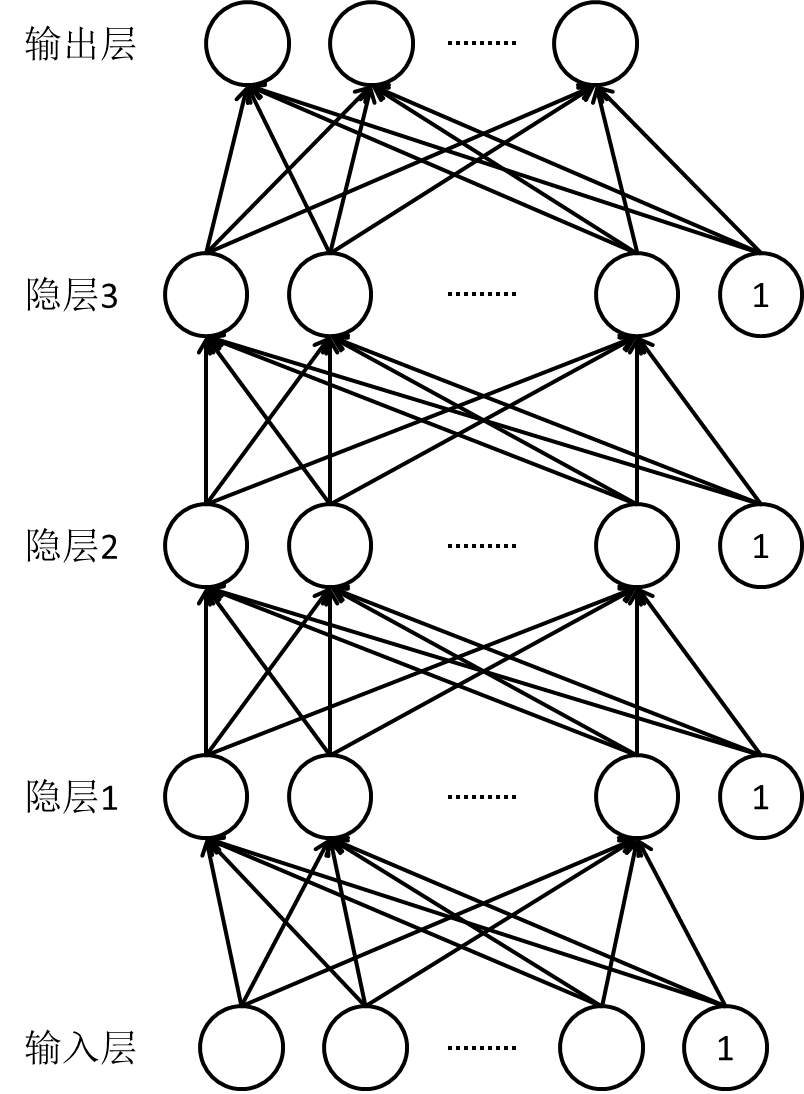
\includegraphics[height=.4\textheight]{figure/dnn.png}
    \bicaption[fig:dnn]{}{深度神经网络}{Fig}{Deep neural network}
\end{figure}
这里我们将DNN的输入层设为层0,将输出层设为层L。神经网络运算可以被定义为:
\begin{equation}
    \mathbf{y}^l=f(\mathbf{x}^l)=f(\mathbf{W}^l\mathbf{y}^{l-1}+\mathbf{b}^l), 0 < l < L
\end{equation}
这里$\mathbf{x}^l, \mathbf{y}^l, \mathbf{W}^l, \mathbf{b}^l$分别是第$l$个隐层的输入向量、输出向量、权重矩阵和偏置向量。$\mathbf{y}^0=\mathbf{o}$是网络输入特征向量。$f$是一种对输入向量进行元素级计算的激活函数。常用激活函数有:
\begin{itemize}
    \item sigmoid函数
    \begin{equation}
        f(x)=\sigma(x)=\frac{1}{1+e^{-x}}
    \end{equation}
    \item 双曲正切函数
    \begin{equation}
        f(x)=\text{tanh} (x)=\frac{e^x-e^{-x}}{e^{x}+e^{-x}}
    \end{equation}
    双曲正切函数是sigmoid函数的调整版本,它们具有相同建模能力。区别是sigmoid函数的值域是(0,1),这有助于得到更稀疏表示。而tanh的值域是(-1,1)是对称,更容易训练。
    \item 整流线性单元(ReLU)
    \begin{equation}
        \text{ReLU}(x)= \max (0,x)
    \end{equation}
    它的导数更加简洁且不会随着层数增多而出现梯度消失现象。
\end{itemize}
如图~\ref{fig:act}所示,其中黑色的曲线为sigmoid;红色曲线为tanh;蓝色的曲线为ReLU。因为sigmoid函数被应用得更加广泛,在本文中如果没有特别标明,默认都是使用sigmoid函数。
\begin{figure}[!htp]
  \centering
    \captionstyle{\centering}
    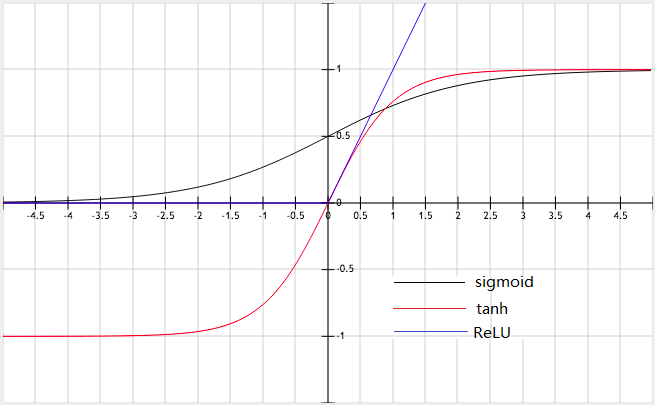
\includegraphics[height=.5\textwidth]{figure/activation.png}
    \bicaption[fig:act]{}{激活函数}{Fig}{Activation functions}
\end{figure}

深度神经网络输出层选定通常根据任务而变化,如果是回归任务,通常使用一个线性层:
\begin{equation}
    \mathbf{y}^L=\mathbf{x}^L=(\mathbf{W}^L)^{\top}\mathbf{y}^{L-1}+\mathbf{b}^L
\end{equation}
如果是多分类的任务,通常会使用输出层每个神经元代表一类,其中第$i$个神经元的值即代表了当前特征属于类别$i$概率,因此它必须满足多项式分布,即$y^L_i \ge 0$且$\sum_{i=1}^C y_i^L=1$,这里$C$为总类别数。为了满足这一限制,我们通常会使用softmax函数进行归一化:
\begin{eqnarray}
    y_i^L&=&P_{\text{dnn}}(i|\mathbf{o})=\text{softmax}_i(\mathbf{x}^L) \\
    &=& \frac{e^{x_i^L}}{\sum_{j=1}^C e^{x_j^L}}
\end{eqnarray}
给定了特征向量的输入后,DNN输出由模型参数$\mathcal{M}=\{ \mathbf{W}^l, \mathbf{b}^l, 0 < l \le L\}$确定,通过使用前面提到的公式计算输出向量以及最后输出,这一过程也被称为前向计算。

\subsubsection{卷积神经网络}
传统的深度卷积神经网络(convolutional neural network, CNN)~\cite{lecun1998gradient}通常由若干卷积层和池化层组成,最后接上一些全连接层。和深度神经网络相比,它主要区别在于卷积层和池化层。本章将具体介绍卷积层和池化层。

特征图谱是卷积层和池化层中最基本的单元,每个卷积层输入和输出都是若干张特征图谱。在语音识别中,包含静态特征、一阶和二阶动态特征的经典语音信号的特征可以表示为三张特征图谱。每张特征图谱是一张大小为$N_t \times N_f$的图片,通常为$11 \times 40$。这里$N_t$是上下文窗口大小,$N_f$是提取特征的维度。相比于MFCC或者PLP特征,FBANK特征更适合CNN。首先FBANK特征中各个维度之间是相关的,这种相关性可以被卷积进行捕捉。其次,池化操作中降采样需在一个有序的频率特征图谱中进行才有意义。MFCC特征中的离散余弦变换将破坏这些性质。

\begin{figure}[!htp]
  \centering
    \captionstyle{\centering}
    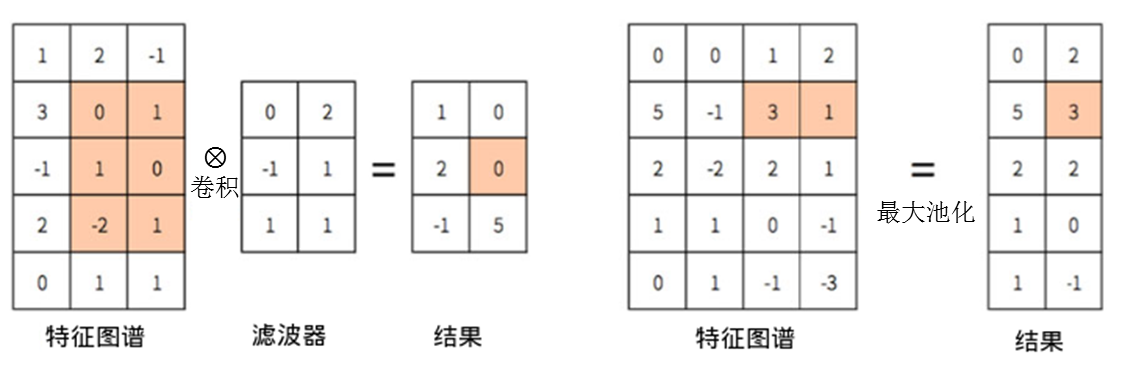
\includegraphics[width=.8\textwidth]{figure/cnn.png}
    \bicaption[fig:cnn]{卷积操作和池化操作}{卷积操作和池化操作,左边为卷积,右边为最大池化}{Fig}{Convolution and pooling, (left: convolution, right: max pooling)}
\end{figure}

卷积操作可以视为在特征图谱上使用一个滤波器。特征图谱和滤波器都可以通过矩阵表示。卷积过程就是将滤波器从特征图谱的左上角逐行扫描到右下角。在这一过程中被滤波器覆盖到的区域被称为感受野。在每一步中,感受野会将滤波器和它所覆盖到的特征图谱区域进行点乘得到一个输出值,将整张特征图谱扫描完后即可得到输出特征图谱,卷积数学定义为:
\begin{eqnarray}
    \mathbf{y} &=& \mathbf{w} \otimes \mathbf{x} \\
    y_{i,j} &=& \sum_{a=1}^A \sum_{b=1}^B W_{ab} x_{i+a-1, j+b-1} \\
    0 < &i& \le W-A+1 \\
    0 < &j& \le H-B+1 \\
\end{eqnarray}
其中$W$是大小为$A \times B$的二维滤波器,$\mathbf{x}$是大小为$W \times H$输入特征图谱,$\mathbf{y}$是大小为$W-A+1 \times H-B+1$的输出特征图谱。
如图~\ref{fig:cnn}中左边部分所示为卷积操作的图例,图中输入为一个$5 \times 3$特征图谱,滤波器大小为$3 \times 2$,最后得到一个$3 \times 2$输出特征图谱。

整个卷积层可以由如下公式表示:
\begin{equation}
    \mathbf{y}^{l}_{i} = \sigma ( \sum_{j=1}^{N} ( \mathbf{w}^{l}_{i,j} \otimes \mathbf{y}^{l-1}_{j} ) \oplus b^{l}_{i} )
\end{equation}

这里$\mathbf{y}^{l}_i, \mathbf{y}^{l-1}_j$分别是第$l$个卷积层的第$j$个输入特征图谱和第$i$个输出特征图谱。$\mathbf{W}^l_{i,j}$是这两个特征图谱间滤波器。$b^l_i$是一个应用于整张特征图谱偏置值,$\otimes$为卷积操作,$\oplus$表示特征图谱中每个元素都加上相同的值$b^l_i$。$\sigma$是激活函数,通常使用sigmoid或者ReLU。$N$是输入特征图谱个数。由于各个感受野之间的参数是共享的,因而CNN中参数个数相对DNN是很少的。

池化层通常扮演降采样功能,它输入若干特征图谱并输出降低了分辨率后特征图谱。本文使用了最大值池化方法,一个$1 \times 2$的最大值池化效果如图~\ref{fig:cnn}中的右边部分所示。

\subsubsection{循环神经网络}
循环神经网络(recurrent neural network, RNN)是深度神经网络一个变种,在建模时序数据中特别有效。与前馈网络不同点在于它包含有一条回环,在循环神经网络中,隐层在时刻$t$输出不仅仅作为下一层的输入,同时也会在时刻$t+1$输回给自身。因此它相当于存在内部状态,内部状态将过去历史信息进行了编码。最简单的循环神经网络可以被描述为:
\begin{equation}
    \mathbf{y}^l_t = \sigma(\mathbf{W}^l_y \mathbf{y}^{l-1}_t + \mathbf{W}^l_h \mathbf{y}^l_{t-1} + \mathbf{b}^l)
\end{equation}
这里$\mathbf{y}^l_t$是网络第$l$层第$t$帧的隐层输出,$\mathbf{W}^l_y, \mathbf{W}^l_h$分别是用于对上层输出和对历史输出权重矩阵。

通过这一设计,神经网络可以使用所有的过去帧的信息,上下文信息在声学模型建模中扮演了很重要的作用。在~\cite{graves2013hybrid,graves2013speech,sak2014long,sak2014sequence}中,作者使用了深度循环神经网络来建模声学模型。双向循环神经网络也被用于语音识别,它不仅能捕捉过去历史信息,也能捕捉未来的整个输入序列信息。

在早期的工作中,RNN层仅仅使用了一个线性变换接上一个元素级激活函数,这种结构没法保留长时信息,因为通用的激活函数会对动态范围进行压缩,因此在$n$帧之前历史信息在到达当前帧时已经被压缩了$n$次,很难对当前决策产生影响。在使用沿时误差反向传播算法中,这一问题也被称为梯度消失问题~\cite{bengio1994learning},即误差无法沿着时间维传播太多帧。为了解决这一问题,在~\cite{hochreiter1997long}中,长短时记忆循环神经网络(long short-term memory, LSTM)被提出用来取代传统的RNN结构。它通过引入记忆单元和门操作来避免梯度消失问题,一个典型的LSTM可由如下公式描述:
\begin{eqnarray}
    \label{eq:lstm}
    \mathbf{i}^l_t &=& \sigma( \mathbf{W}^l_{yi} \mathbf{y}^{l-1}_t + \mathbf{W}^l_{hi} \mathbf{y}^l_{t-1} + \mathbf{w}_{ci} \mathbf{c}^l_{t-1} + \mathbf{b}^l_i) \\
    \mathbf{f}^l_t &=& \sigma( \mathbf{W}^l_{yf} \mathbf{y}^{l-1}_t + \mathbf{W}^l_{hf} \mathbf{y}^l_{t-1} + \mathbf{w}_{cf} \mathbf{c}^l_{t-1} + \mathbf{b}^l_f) \\
    \mathbf{c}^l_t &=& \mathbf{f}^l_t \odot \mathbf{c}^l_{t-1} + \mathbf{i}^l_t \odot \text{tanh}(\mathbf{w}_{yc} \mathbf{y}^{l-1}_t + \mathbf{w}_{hc} \mathbf{c}^l_{t-1} + \mathbf{b}^l_c) \\
    \mathbf{o}^l_t &=& \sigma( \mathbf{W}^l_{yo} \mathbf{y}^{l-1}_t + \mathbf{W}^l_{ho} \mathbf{y}^l_{t-1} + \mathbf{w}_{co} \mathbf{c}^l_{t-1} + \mathbf{b}^l_o) \\
    \mathbf{y}^l_t &=& \mathbf{o}^l_t \odot \text{tanh}(\mathbf{c}^l_t)
\end{eqnarray}
和循环神经网络一样,它需要从第一帧开始迭代进行前向传播,这里$\sigma$是非线性sigmoid函数,$\mathbf{i}^l_t, \mathbf{f}^l_t, \mathbf{o}^l_t, \mathbf{c}^l_t, \mathbf{y}^l_t$分别是第$t$帧的输入门、遗忘门、输出门、记忆单元和隐层输出。$\odot$表示元素级乘法。$\mathbf{w}_*, \mathbf{b}_*$分别是权重矩阵和偏置,其中$\mathbf{w}_{ci}, \mathbf{w}_{cf}, \mathbf{w}_{co}$是对角矩阵。与最初的LSTM结构不同之处在于,在这一结构中我们增加了窥孔连接(peephole connection)。即:将记忆单元的状态同时输入给各个门操作。

在大词汇连续语音识别任务中,按照~\cite{sak2014long}中建议,通常会使用一个投影层来降低计算量(Long Short-Term Memory with Projection, LSTMP)。它和公式~\ref{eq:lstm}的主要区别是在输出$\mathbf{y}^l_t$上增加一个线性变换来降低维度,即:
\begin{equation}
    \mathbf{y}^l_t = \mathbf{w}_{r} ( \mathbf{o}^l_t \odot \text{tanh}(\mathbf{c}_t) )
\end{equation}

\subsection{神经网络训练}
\subsubsection{训练准则}
在DNN训练中通常有两个常用的准则,对于回归任务常使用均方误差(mean square error, MSE)准则:
\begin{equation}
    \mathcal{F}_{\tt MSE}(\mathcal{M}) = \frac{1}{T}\sum_{t=1}^T \lVert \mathbf{y}_t^L - \bar{\mathbf{y}}_t \rVert^2_2
\end{equation}
这里$\mathbf{y}_t^L$是由神经网络估计出输出, $\bar{\mathbf{y}}_t$是正确标注。

对于分类任务而言,正确的标注为一个概率分布,通常使用交叉熵(cross entropy, CE)来进行优化:
\begin{equation}
    \mathcal{F}_{\tt CE}(\mathcal{M}) = - \frac{1}{T}\sum_{t=1}^T \sum_{c=1}^C \bar{y}_t(c) \log y_t^L(c)
\end{equation}
这里$\bar{y}_t(c)$是标注中类$c$概率,$y_t^L(c)$是神经网络估计出的类$c$概率。最小化交叉熵准则等价于最小化标注分布与DNN估计分布之间的KL距离(Kullback-Leibler divergence, KLD)。一般,研究者通常使用硬标注作为标注分布,即:
\begin{equation}
    \bar{y}_t(c) = 
    \begin{cases} 
        1& c=l_t \\ 
        0& c \ne l_t 
    \end{cases}
\end{equation}
这里$l_t$是第$t$帧标注。此时,CE准则退化为负对数似然准则(negative log-likelihood, NLL)
\begin{equation}
    \mathcal{F}_{\tt NLL}(\mathcal{M}) = -\log y^L_t(l_t)
\end{equation}

\subsubsection{反向传播算法}
给定了训练准则后,可通过著名的误差反向传播(error back-propagation, BP)~\cite{rumelhart1986learning}算法来进行参数优化。由于BP算法基于梯度下降方法来更新模型参数,因而其中的关键步骤是使用链式法则进行梯度计算。

最顶层权重矩阵的梯度取决于所使用训练准则。对于回归问题,当使用MSE的训练准则时,输出层权重矩阵的梯度是
\begin{eqnarray}
    \frac{\partial \mathcal{F}_{\tt MSE}(\mathcal{M}))}{\partial W^L_{ij}} &=& \frac{\partial \mathcal{F}_{\tt MSE}(\mathcal{M}))}{\partial x^L_j} \frac{\partial x^L_j}{\partial W^L_{ij}} \\
    &=& e^L_j \frac{\partial x^L_j}{\partial W^L_{ij}} \\
    &=& (x^L_j - \bar{y}_j) y^{L-1}_i
\end{eqnarray}
这里$e^L_j$为误差信号:
\begin{equation}
    \mathbf{e}^L \triangleq [ \frac{\partial \mathcal{F}_{\tt MSE}(\mathcal{M}))}{\partial x^L_1}, \dots, \frac{\partial \mathcal{F}_{\tt MSE}(\mathcal{M}))}{\partial x^L_N} ]^{\top}
\end{equation}
$N$是最后一层输出维度。
也可以将对$\mathbf{W}^L$梯度写为矩阵形式:
\begin{equation}
   \nabla_{\mathbf{W}^L} \mathcal{F}_{\tt MSE}(\mathcal{M})) = \mathbf{e}^L {\mathbf{y}^{L-1}}^{\top} = (\mathbf{x}^L - \bar{\mathbf{y}}) {\mathbf{y}^{L-1}}^{\top}
\end{equation}
当使用分类任务时,CE准则通常和softmax输出层一起使用,同样先计算出误差信号:
\begin{eqnarray}
    e^L_j &=& \frac{\partial \mathcal{F}_{\tt CE}(\mathcal{M}))}{\partial x^L_j} = - \frac{\partial \sum_{c=1}^C \bar{y}_c \log \text{softmax}_c(\mathbf{x}^L) }{\partial x^L_j} \\
    &=& \frac{\partial \sum_{c=1}^C \bar{y}_c \log \sum_{i=1}^C e^{x^L_i} }{\partial x^L_j} - \frac{\partial \sum_{c=1}^C \bar{y}_c \log e^{x^L_c} }{\partial x^L_j} \\
    &=& \frac{e^{x^L_j}}{\sum_{i=1}^C e^{x^L_i}} - \bar{y}_j \\
    &=& y^L_j-\bar{y}_j
\end{eqnarray}
接着可以求出对$\mathbf{W}^L$的梯度:
\begin{equation}
    \nabla_{\mathbf{W}^L} \mathcal{F}_{\tt CE}(\mathcal{M})) = (\mathbf{y}^L - \bar{\mathbf{y}}) {\mathbf{y}^{L-1}}^{\top}
\end{equation}
值得注意一点是,虽然CE准则和MSE准则梯度公式看上去有相同的形式,但实际上它们是不同的,因为在做回归时$\mathbf{y}^L=\mathbf{x}^L$,而在做分类时$\mathbf{y}^L=\text{softmax}(\mathbf{x}^L)$。

对于非顶层权重矩阵的梯度$0<l<L$,则有:
\begin{eqnarray}
    \frac{\partial \mathcal{F}(\mathcal{M}))}{\partial W^l_{ij}} &=& \frac{\partial \mathcal{F}(\mathcal{M}))}{\partial x^l_j} \frac{\partial x_j^l}{\partial W^l_{ij}} \\
    &=& e^l_j \frac{\partial x^l_jL}{\partial W^l_{ij}} \\
    &=& e^l_j y^{l-1}_i
\end{eqnarray}
这里$\mathbf{e}^l \triangleq \nabla_{\mathbf{x}^l} \mathcal{F}(\mathcal{M})$是对第$l$层的激励误差信号:
\begin{eqnarray}
    e^l_i &=& \frac{\partial \mathcal{F}(\mathcal{M})}{\partial x^l_i} \\
    &=& \sum_{j=1}^{N^{l+1}} \frac{\partial \mathcal{F}(\mathcal{M})}{\partial x^{l+1}_j} \frac{\partial x^{l+1}_j}{\partial y^l_i} \frac{\partial y^{l}_i}{\partial x^l_i} \\
    &=& \sigma'(x^{l}_i)  \sum_{j=1}^{N^{l+1}} e^{l+1}_j W^{l+1}_{ji}
\end{eqnarray}
这里$N^{l+1}$是第$l+1$层隐层节点数,写出矩阵形式即:
\begin{equation}
    \label{eq:error_prop}
    \mathbf{e}^l = ( {\mathbf{w}^{l+1}} \mathbf{e}^{l+1} ) \odot \sigma'(\mathbf{x}^l)
\end{equation}
这里$\odot$为元素级相乘,$\sigma'(x^l_j)$为激活函数的元素级导数,对于sigmoid函数,它等于:
\begin{equation}
    \sigma'(x^l_j)=(1-y^l_j)y^l_j
\end{equation}
令$\sigma'(\mathbf{x}^l) = [\sigma'(x^l_1), \dots, \sigma'(x^l_{N^l})]^{\top}$。

因此对权重矩阵梯度矩阵形式为:
\begin{equation}
    \nabla_{\mathbf{W}^l} \mathcal{F}(\mathcal{M}) = \mathbf{e}^l {\mathbf{y}^{l-1}}^{\top}
\end{equation}
从公式\ref{eq:error_prop}中可以观察到,误差信号需要自顶层向下进行反向传播,因此该方法被称为误差反向传播算法。

\subsubsection{神经网络的优化}
\label{sec:intro-sgd}
深度神经网络采用梯度下降的方法进行优化,因此每一轮迭代都需要对一个批量(batch)训练样本计算梯度,称为{\em 小批量随机梯度下降}。批量大小的选择上通常海会同时影响收敛速度与模型的性能。

最简单批量选择方法是去使用整个训练集,这种方法被称为批量训练(batch training)。它有如下优势:首先,批量训练的收敛性是众所周知的,其次,批量训练可以在多计算机之间并行。但由于每次参数更新都要遍历全部数据集~\cite{yu2010roles},所以对大词汇语音识别任务而言,这是十分低效的。

另外一种选择是随机梯度下降法(Stochastic gradient decent, SGD)~\cite{bottou1998online},在机器学习领域也被称作在线学习。SGD根据从单个训练样本估计出的梯度来更新模型参数~\cite{yu2010roles}。如果样本点是独立同分布的(在训练数据中随机采样很容易达成),可以证明这种方法是对梯度的无偏估计,只不过存在噪声。这点虽然看似不利,实则是SGD相比批量算法优势所在:由于DNN是高度非线性的且优化准则也是非凸的,因而目标函数包含很多局部最优,而SGD估计中存在噪声,从而使得其能从局部最优中跳出来进入一个更好全局最优。

SGD通常比批量训练快很多,特别是在大词汇连续语音识别中。这是因为在大数据集中,通常有很多样本是相似甚至重复的,所以用全部数据集来计算梯度是浪费的。然而,由于SGD只计算一个样本梯度,无法高效的利用GPU的并行能力,且因为噪声的存在无法完全收敛至局部最优点,所以通常会使用SGD和批量训练折中方案,小批量(mini-batch)训练~\cite{yu2010roles}。小批量数据通过从训练样本中抽取一小组数据来计算梯度使得其可以高效的使用GPU的并行能力,并且也拥有SGD跳出局部最优的性质。

惯性系数~\cite{polyak1964some}是优化中一种加速收敛的方法,它主要思想是使用过往梯度的一个累积量和当前梯度的插值作为最终更新使用的梯度,即:
\begin{eqnarray}
    \Delta\mathbf{W}^l_p = \rho \Delta \mathbf{W}^l_{p-1} + (1-\rho) \frac{1}{M} \sum_{m=1}^M \nabla_{\mathbf{W}^l_p} \mathcal{F}(\mathcal{M}, \mathbf{o}_m, \bar{\mathbf{y}}_m)
\end{eqnarray}
这里,$\nabla_{\mathbf{W}^l_p} \mathcal{F}(\mathcal{M}, \mathbf{o}_m, \bar{\mathbf{y}}_m)$是使用样本$\mathbf{o}_m, \bar{\mathbf{y}}_m$计算出的梯度。$\Delta\mathbf{W}^l_p$是第$p$轮迭代累积的梯度。$\rho$即为惯性系数。使用惯性系数会令参数更新变得更加平滑,同时减少梯度估计时方差,因此可以加速训练。

\subsubsection{参数初始化与预训练}
通常有很多启发式的方法来初始化DNN模型,它们的主要思想都是希望初始化后的激活范围处于sigmoid函数的线性段。即激活值为0.5左右。如果权重过大将导致激活值趋近于0或者1,这样计算出梯度就会非常小。随机初始化的另外一个作用是打破深度神经网络的对称性。在~\cite{lecun1998efficient}中,Lecun建议从一个均值为0,方差为$\frac{1}{\sqrt{N^l}}$的高斯分布中采样。由于在语音识别中隐层节点的个数通常从1000至2000不等,所以一般选取[-0.05, 0.05]的均匀分布作为权重矩阵的初始化,而偏置初始化为0。

由于DNN模型高度非线性和非凸性,研究者通常会使用一些预训练的方法使其能从一个更优的初始值开始优化。最著名的两个预训练方法是深度置信网络和鉴别性预训练。

深度置信网络(Deep belief network, DBN)是由多层受限玻尔兹曼机(restricted Boltzmann machine, RBM)组成生成性模型。

\begin{figure}[!htp]
  \centering
    \captionstyle{\centering}
    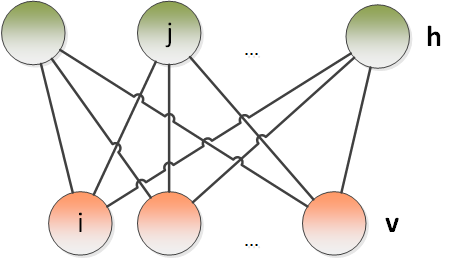
\includegraphics[width=.4\textwidth]{figure/RBM.png}
    \bicaption[fig:rbm]{}{受限玻尔兹曼机}{Fig}{Restricted Boltzmann machine}
\end{figure}

受限玻尔兹曼机是一种生成性模型,它是玻尔兹曼机的一个变种。它结构如~\ref{fig:rbm}所示~\footnote{图片引用自~\cite{ASRBook-Yu2014}},它取消了玻尔兹曼机中可见层神经之间和隐藏层神经之间的连接。因此,它形成了一张二分图。

在RBM中,由于隐层神经元之间没有连接,因而可见层神经元之间也没有连接~\cite{yu2010roles}。所以,可以很方便计算后验概率。
将多个RBM网络自底向上逐层堆叠就得到了深度信念网络,在深度信念网络中每一层的输出都作为后一层的输入,然后用新特征继续训一个RBM。最终DBN训练完成后将DBN中的权重直接作为DNN网络初始化。

使用DBN进行预训练有如下潜在优势:
\begin{itemize}
    \item DNN是高度非线性且非凸的,初始化点会很大程度影响最终模型。
    \item 预训练阶段使用的是生成性准则与反向传播算法中使用的鉴别性准则不同~\cite{yu2010roles},因此潜在对模型进行了正则化。
    \item 在预训练时可以利用大量的无标注数据。
\end{itemize}

DNN的参数也可以使用鉴别性预训练(discriminative pretrain, DPT)来鉴别性地初始化,即逐层进行BP。鉴别性预训练流程如下: 首先使用标注鉴别性训练一个单隐藏层的DNN若干轮(并不需要训练到收敛),接着在最后一个隐层和输出层之间插入一个新的随机初始化的隐藏层,并且鉴别性训练整个网络若干轮,直至达到期望的层数。预训练目标是希望网络能从一个更优秀的初试点开始进行训练以潜在地改善神经网络鲁棒性。然而,当训练数据足够大(大于15小时)或者使用ReLU作为激活函数之后,预训练带来性能提升就不那么明显了。

\subsection{深度神经网络-隐马尔科夫模型混合系统}
\label{sec:dnn_hmm}

\begin{figure}[!htp]
  \centering
    \captionstyle{\centering}
    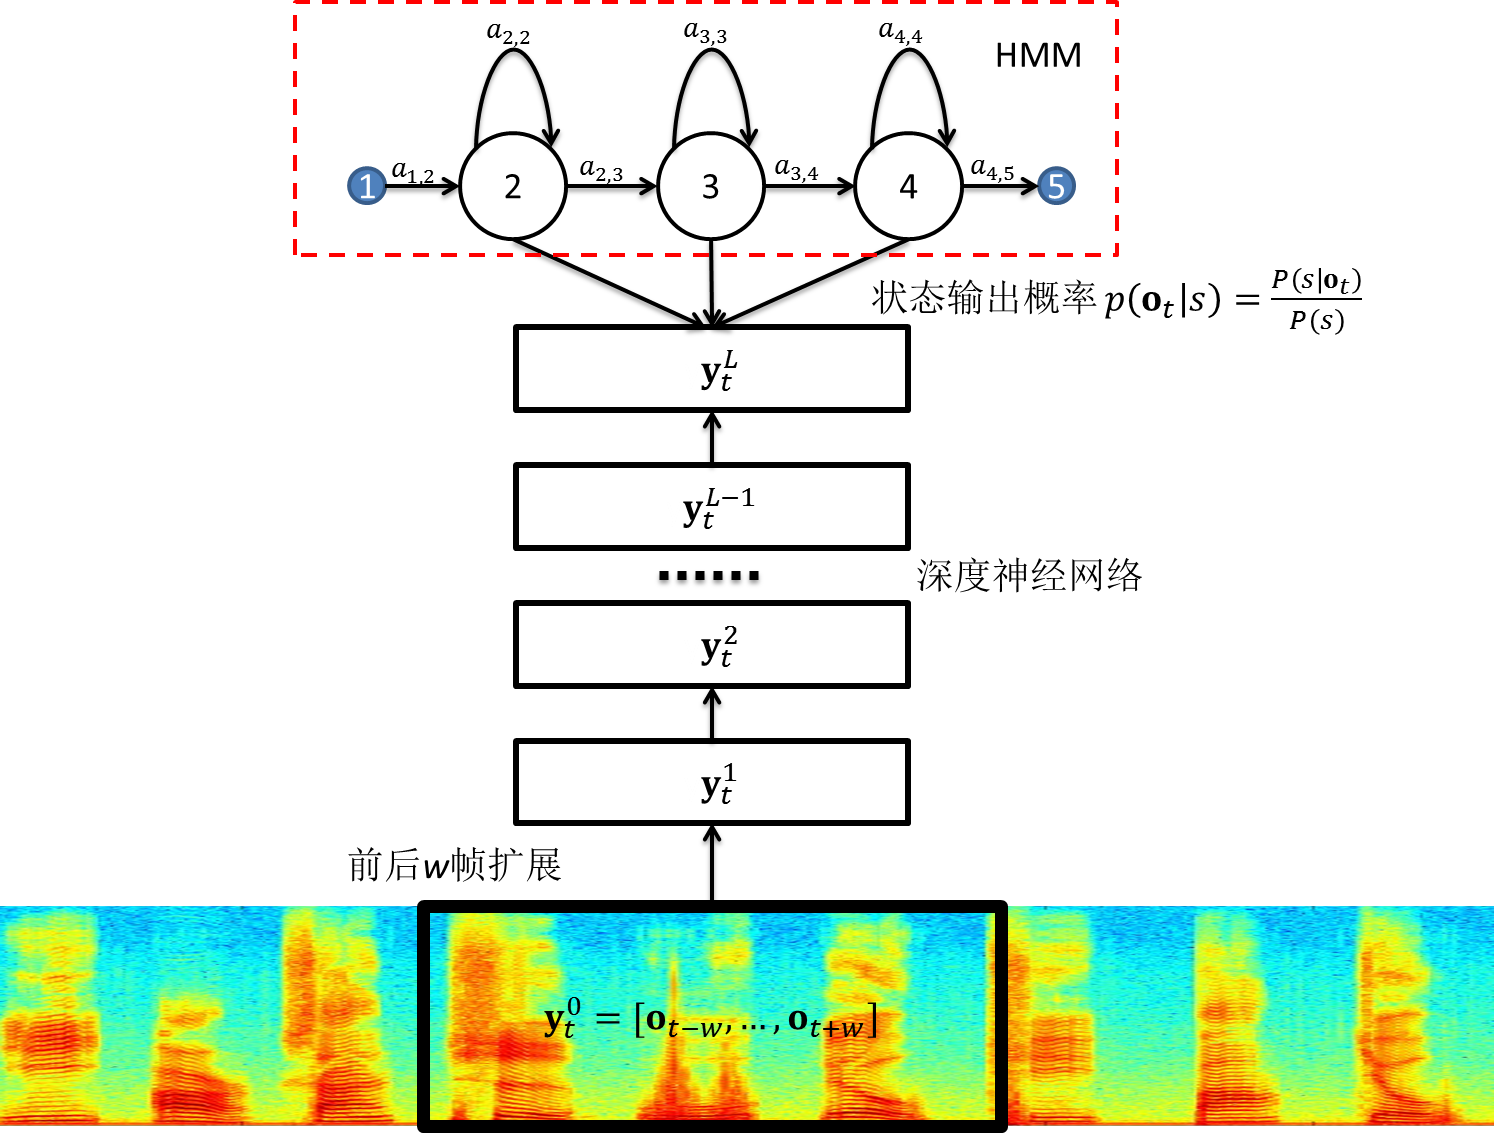
\includegraphics[width=.618\textwidth]{figure/dnn_hmm.png}
    \bicaption[fig:dnn-hmm]{}{DNN-HMM混合系统}{Fig}{Structure of DNN-HMM hybrid system}
\end{figure}

在前文介绍的深度神经网络并不能直接为语音信号的信号建模,这是由于语音信号处理的信号是一种时序连续信号,而深度神经网络的输入是固定大小的向量。早在20世纪80年代末就已经有研究提出了结合人工神经网络(ANN)和HMM方法用于语音识别~\cite{trentin2001survey}。目前有效的方法是如图\ref{fig:dnn-hmm}中所描绘的DNN-HMM混合系统。在这一框架中,HMM被用于描述语音信号的信号动态变化,而DNN则用于估计语音信号的特征向量的输出概率,通常是用来估计给定观测语音信号的特征后,该特征由HMM中某个状态释放后验概率。换句话说,DNN只是替代了GMM在公式(\ref{eq:hmm-basic})中对$p(\mathbf{O}|\mathbf{s},\mathcal{M})$的建模。

DNN-HMM的优点在于它能方便的利用DNN内在的鉴别性能力,另外训练过程可以直接使用维特比算法,解码过程不需要有特别改变。

在~\cite{bourlard1989continuous,bourlard1989links,morgan1990continuous}中,该方法被称为ANN-HMM混合模型,它只使用了上下文无关音素状态之间且仅用于小词汇语音识别。随后在~\cite{bourlard1992cdnn}中被扩展为上下文相关的音素建模,以及被用于LVCSR任务~\cite{robinson2002connectionist}。但是,因为过去计算能力有限,通常只使用了两层隐层的神经网络,所在并没有比GMM-HMM框架取得更好性能。

最近的技术发展~\cite{CD-DNN-HMM-dahl2012,DNN4ASR-hinton2012,seide2011conversational,yu2010roles}则说明,如下几个改变可以使其获得更重大识别性能提升。
\begin{itemize}
    \item 首先,使用更深的深度神经网络,比如拥有6个隐层DNN。
    \item 其次,使用语素(即状态聚类后的三音素状态)来代替单音素状态作为深度神经网络的输出单元。这一模型被称为上下文相关的深度神经网络隐马尔科夫模型(Context-dependent pre-trained deep-neural-network hidden markov model, CD-DNN-HMM)。直接使用语素还有一个额外好处,即它对CD-GMM-HMM系统修改最小。
\end{itemize}
在CD-DNN-HMM中。对于所有的状态$s \in [1,S]$中只有一个完整的DNN来估计状态后验概率$P(s_t=s|\mathbf{o}_t)$。这和传统的GMM是不同的,在GMM中,我们使用不同GMM来对不同的状态建模。除此之外,典型的DNN输入不是单独一帧,而是一个$2w+1$帧大小窗口特征$\mathbf{y}^0_t= [ \mathbf{o}_{t-w}^{\top}, \dots, \mathbf{o}^{\top}_t, \dots, \mathbf{o}^{\top}_{t+w} ]^{\top}$

在解码过程中,因为HMM需要使用似然度$p(\mathbf{o}_t|s_t)$而非后验概率,所以我们需要将后验概率转为似然度:
\begin{equation}
    \label{eq:dnn}
    p(\mathbf{o}_t|s_t=s) = \frac{P(s_t=s|\mathbf{o}_t)p(\mathbf{o}_t)}{P(s)}
\end{equation}
其中,$p(s)=\frac{T_s}{T}$是从训练集中统计出的每个状态先验概率。$T_s$是状态$s$的帧数,$T$是总帧数。因为$p(\mathbf{o}_t)$是与词序列无关的,计算时可忽略。所以最终似然可以通过$p(\mathbf{o}_t|s_t=s)=\frac{P(s_t=s|\mathbf{o}_t)}{P(s)}$计算。

CD-DNN-HMM训练可以使用维特比算法来进行,CD-DNN-HMM包含了三个组成部分,深度神经网络DNN,隐马尔科夫模型HMM和GMM-HMM系统中的状态绑定结构的状态。所以CD-DNN-HMM第一步是去使用训练数据训练一个GMM-HMM,然后在该系统上使用维特比算法获得状态级的强制对齐,同时保留该系统中的状态转移概率和状态映射关系,接着使用由GMM-HMM系统计算得到状态对齐(state alignment)作为标注使用CE准则训练一个DNN。最后,解码时使用公式~\ref{eq:dnn}来得到似然进行解码。



\section{基于深度学习的序列建模}
\label{Sec:seq-tr-review}

由于语音识别本身是一个序列预测问题,所以序列级的准则往往能够带来性能的提升。依据序列的不同建模方式,目前有两种不同的序列鉴别性训练方法,一种针对  生成式序列模型 (Generative Sequence Model, GSM) 比如上文介绍的HMM以及其相应的深度学习系统;另一种则针对 鉴别式序列模型 (Discriminative Sequence Model, DSM) ,比如 CTC,Encoder-decoder模型等。 
%序列鉴别性训练 for GSM is discussed in Section~\ref{Sec:sgm-sdt-intro} and DSM based 序列鉴别性训练 is discussed in Section~\ref{Sec:sdm-sdt-intro}.
 %while 序列鉴别性训练 in  CTC framework is considered in Section~\ref{Sec:kws-ctc}.

%table to show 
%       frame seq
%gen
%disc


\subsection{生成式序列模型和鉴别式序列模型}
\label{Sec:sgm-and-sdm}
在语音识别中一个独有并且有趣的自然现象是声学序列和语言学序列的长度可变性。
该任务中,在训练阶段,一组带有已知标签的输入特征被提供给系统进行模型构建;而测试阶段,则基于特征序列和其它知识源如语言模型和字典进行模型推理搜索。序列标注问题与传统模式分类框架的区别在于以下两个方面。
\begin{itemize}
\item 序列内数据的相关性。无论是特征序列,还是标签序列,序列中各数据点均不符合独立同分布(i.i.d.)假设。特征序列是由声道的连续运动而产生的。而标签序列则受到句法和语法规则、字典以及语言模型的约束。因此,特征和标签均为强相关序列。

\item 标签和特征序列之间的相关性。ASR中,特征和标签之间的对齐方式是未知的,标签序列总是短于特征序列,即其主要问题在于由语速变化等导致的特征序列的可变长性。这就要求序列模型能够同时确定输出序列的位置和内容。
\end{itemize}

如果我们定义语音识别所要建模的输出序列为$\mathbf w$,特征输入序列为 ${\mathbf O}$,
那么为了对上述序列$\mathbf w$与${\mathbf O}$的相关特征进行建模,人们提出了序列模型。下文中我们将首先给出序列模型的定义方式,而后在第\ref{Sec:sgm-sdt-intro}章节和第\ref{Sec:sdm-sdt-intro}章节讨论这些模型在语音识别任务中如何进行序列建模。

通常来说,出于以下原因,序列模型被分解为帧层面的训练准则:1)为了更加高效地发挥帧层面分类器的建模效果,如高斯混合模型(Gaussian mixture model, GMM~\cite{woodland1994large})和深度神经网络(deep neural network, DNN ~\cite{hinton2012deep});2)为了减轻模型的稀疏性,以及通过将简单模型分解为多个组分来增强模型的泛化能力,例如ASR中将模型分解为声学模型、字典和语言模型等;3)未经序列分解的模型在推理搜索前需要得到整个序列信息进而进行后续处理,这将给解码过程造成严重的运行延时。本文提出的序列标注方法即是基于帧层面分解的模型~\cite{forney1973viterbi,mohri2002weighted}。
因此
大部分序列模型都包含一个用来对时序特性建模的部分, 比如GMM~\cite{woodland1994large} 和深度学习模型~\cite{hinton2012deep}用来对局部的声学特征进行建模,再加上一个对序列长度和转移进行建模的部分,比如HMM。近期提出的鉴别式序列模型, encoder-decoder~\cite{chan2016end}则尝试直接对序列建模而不是进行序列到逐帧的拆分。但在大部分语音识别研究中,性能和延迟在上述模型中都有一定限制。因此不参与本章节讨论。
本章节所有的序列鉴别性训练方法均基于逐帧的分解方式。

概率模型通常可以分为生成式和鉴别式两种类型,由此序列模型的区别在于对条件似然度或者后验概率进行建模。
但无论哪一种模型,最终都是为了对完整序列进行建模,即给定特征序列,建模输出序列的概率。
值得注意的是在序列上或者在帧上,都可以使用生成式或者鉴别式进行分别建模,二者工作在不同层面上。
比如目前通常使用的混合 NN-HMM 模型就是采用生成式序列模型和鉴别式帧分类器。
在本章节中,我们主要关注序列模型。下文我们将比较模型结构和优化准则,在生成式和鉴别式序列模型中的异同。


{\em 生成式序列模型}(Generative Sequence Model, GSM)通常被定义为条件似然度$p(\mathbf{O}|\mathbf{w})$, 公式中 ${\mathbf O}$ 表示特征输入序列, $\mathbf w$ 表示标签输出序列。隐马尔科夫模型 (HMM) 是这类生成式序列模型的一个经典例子~\footnote{另一类 GSM 例子是Kalman 滤波器~\cite{digalakis1991dynamical,abbeel2005discriminative}.}。
%
当一个序列级鉴别性训练准则,即序列后验概率,被优化时,我们一般采用贝叶斯公式分解来使得生成式模型可以使用鉴别性准则进行优化,我们将在随后的一章节展开讨论。



{\em 鉴别式序列模型}(Discriminative Sequence Model, DSM) 由 $P(\mathbf{w}|\mathbf{O})$进行定义,表示给定特征序列$\mathbf{O}$建模序列 $\mathbf{w}$的后验概率。当使用了序列鉴别性模型之后,序列鉴别性准则的优化形式就非常直接了。 
连接时序分类模型 (CTC)~\cite{graves2006connectionist} 是其中一种鉴别式序列模型. 它引入了 $\tt blank$标签来建模输出序列之间的混淆部分。我们将在第\ref{Sec:sdm-sdt-intro}章节详细介绍CTC的定义方式。
另一类鉴别式序列模型称为基于注意力机制的序列到序列模型(encoder-decoder模型),将在第\ref{chap:intro2-e2e-s2s}章节讨论。


%In summary, sequence models are used to model the temporal characteristics of the acoustic feature sequences. 
%
%They can be divided into 生成式序列模型 and 鉴别式序列模型. 
%Further investigations are given  in Section~\ref{Sec:disc-and-ctc}.

\subsection{基于HMM的传统序列鉴别性训练}
\label{Sec:sgm-sdt-intro}

隐马尔科夫模型 (HMM)是一个序列生成模型,根据前文的介绍,其建模$p(\mathbf{O}|\mathbf{w})$, 所以使用HMM来对序列后验概率$p(\mathbf{w}|\mathbf{O})$建模时,需要利用贝叶斯公式将后验计算转化为用条件概率(即HMM的定义)表达的形式。
\begin{equation}
\label{equ:map-dec}
\begin{split}
P(\mathbf{w}_u|\mathbf{O}_u)=\frac {p(\mathbf{O}_u|\mathbf{w}_u)P(\mathbf{w}_u)}{p(\mathbf{O}_u)}  
%y_{ut}(s^{(r)}_{ut})
\end{split}
\end{equation}
公式中$\mathbf{w}_u$ 是句子 $u$ 对应的词序列。 在语音识别中,$P(\mathbf{w}_u)$ 是语言模型概率。在关键词检测任务中,$P(\mathbf{w}_u)$ 则可以被定义为关键词和非关键词序列的先验概率。
$p(\mathbf{O}|\mathbf{w})$ 是相应的声学部分,由下式得到。
%INTRO: W relation with L
\begin{equation}
\label{equ:lexicon}
\begin{split}
p(\mathbf{O}|\mathbf{w})=\sum_{\mathbf{L}\in\mathcal{L}(\mathbf{w})} p(\mathbf{O}|\mathbf{L})P(\mathbf{L}|\mathbf{w})
%y_{ut}(s^{(r)}_{ut})
\end{split}
\end{equation}
$\mathcal{L}$定义了从词序列 $\mathbf{w}$ 到它的标签序列 $\mathbf{L}$ 的映射, 比如LVCSR中的tri-phone 序列。 $P(\mathbf{L}|\mathbf{w})$ 是发音概率~\cite{chen2015pronunciation},通常由词典和语言模型来决定。

公式中 $p(\mathbf{O}|\mathbf{L})$ 是由HMM中的定义公式(\ref{eq:hmm-basic})给定的。在NN-HMM 混合系统中, 语音信号的动态性使用HMMs 和来自深度学习模型的后验概率进行建模。
\begin{eqnarray}
\label{equ:hmm-model_2}
%\begin{split}
p(\mathbf{O}|\mathbf{L})&=&\!\!\!\!\!\!\sum_{\mathbf{q}\in\mathcal{A}(\mathbf{L})}\!\!\!p(\mathbf{O},\mathbf{q}|{\mathbf L}) =\sum_{\mathbf{q}}\prod_{t=1}^{T} p({\bf o}_{t}|q_t) P(q_t|q_{t-1})\nonumber\\
%y_{ut}(s^{(r)}_{ut})
&\propto&\sum_{\mathbf{q}}\prod_{t=1}^{T} \frac{P(q_t|{\bf o}_{t})}{P(q_t)}P(q_t|q_{t-1})
%\end{split}
\end{eqnarray}
公式中 $\mathbf{L}$ 表示标签序列,比如LVCSR中的tri-phone。
$\mathbf{q}$ 表示HMM状态序列,  $q_t$ 表示在帧 $t$上的HMM状态。 $P(q_t|q_{t-1})$ 表示 HMM 状态转移概率, $P(q_t)$表示状态的先验概率。
$\mathcal{A}$表示由标签序列 $\mathbf{L}$到它的相应HMM状态序列 $\mathbf{q}$之间的映射,
\begin{equation}
\label{equ:a-func_2}
\begin{split}
\mathcal{A}:\mathbb{L}  \mapsto \{ q_0^{(1)},\cdots,q_4^{(1)},\cdots,q_4^{(|\mathbb{L}|)} \}
\end{split}
\end{equation}
$\mathbb{L}$ 表示 $\mathbf{L}$中所有的标签。 $q_s^{(l)}$ 表示第l个HMM的第s个 HMM 状态。
具体来说,每个标签单元,比如 tri-phone, 对应于一个 HMM 模型。
每个HMM模型则包含5个独立的状态,如图~\ref{fig:hmm}所示。
状态后验概率 $P(q_t|{\bf o}_{ut})$是由神经网络来估计得到的。


特征序列 $\mathbf{O}_u$ 的边缘概率 $p(\mathbf{O})$是由所有可能的序列的概率进行求和得到的。
\begin{equation}
\label{equ:po-prob}
\begin{split}
p(\mathbf{O}_u)=\sum_\mathbf{w} p(\mathbf{O}_u,\mathbf{w})= \sum_\mathbf{w} P(\mathbf{w}) p(\mathbf{O}_u|\mathbf{w})
%y_{ut}(s^{(r)}_{ut})
\end{split}
\end{equation}
公式中 $\mathbf{w}$ 表示其中一条竞争的可能路径,具体来说是词图中的一条解码路径。
作为序列鉴别性训练的一个例子,最大互信息准则 maximum mutual information (MMI)~\cite{bahl1986maximum} 如下定义,
%discriminative training formula (P(O) traditional)
\begin{equation}
\label{equ:lvcsr-mmi}
\begin{split}
\mathcal{F}_{\tt{MMI}}%=\sum_{u} \log P(\mathbf{w}_u|\mathbf{O}_u)\\
%=- \sum_{u} \log \frac {p(\mathbf{O}_u|\mathbf{S}_u)^{\kappa}P(\mathbf{w}_u)}{\sum_{\mathbf{w}} p(\mathbf{O}_u|\mathbf{S})^{\kappa}P(\mathbf{w})}  
=\sum_{u} \log \frac {p(\mathbf{O}_u|\mathbf{w}_u)^{\kappa}P(\mathbf{w}_u)}{\sum_{\mathbf{w}} p(\mathbf{O}_u|\mathbf{w})^{\kappa}P(\mathbf{w})}  
\end{split}
\end{equation}
公式中的分布 $P(\mathbf{w}_u|\mathbf{O}_u)$, 在 (\ref{equ:map-dec})中定义, 并被添加了一个常量 $\kappa$ 进行语言模型的权重调节。 %$\mathbf{S}$ and $\mathbf{S}_u$ is the acoustic model state sequences corresponding to $\mathbf{w}$ and $\mathbf{w}_u$ respectively. 
在公式(\ref{equ:lvcsr-mmi})中给定了序列后验概率表达式, 而其它一些序列鉴别性训练准则则是由贝叶斯风险框架推导得到的,将在接下来的章节中进行讨论~\ref{Sec:lfmmi-train}。


%the key is use LATTICE 
上面提到的序列竞争可能路径 $\mathbf{w}$ 在 (\ref{equ:po-prob})中可以得到,与语言模型一起进行联合解码。解码得到的词图作为一种搜索空间的紧致表示,可以用于计算公式(\ref{equ:po-prob})中的边缘概率 $p(\mathbf{O}_u)$ 。

  
%traditional GMM-HMM based systems achieve significantly better performance when trained using sequence discriminative criteria like WB-MVE~\cite{sukkar1996utterance},  discriminatively trained sub-word verification function~\cite{sukkar1996vocabulary}, MCE~\cite{sandness2000keyword} and performance-related discriminative training~\cite{keshet2009discriminative}.



\subsection{无词图序列鉴别性训练}
\label{chap:intro2-e2e-lfmmi}

第\ref{Sec:seq-tr-review}章节所讨论的传统序列鉴别性训练系统是一种比较经典的序列建模方法,但存在几方面缺陷:
\begin{itemize}
\item 词图构建引入了一个额外的步骤,使得词图更新频度和词图质量需要进行额外的权衡。词图用于对搜索空间进行限制,因此较准确的方法是使用本次模块更新迭代之前的原始模型来生成词图,再依托该词图在进行模型更新迭代。但是每次生成词图需要联合语言模型进行语音识别解码,计算复杂度较大。因此传统序列建模方法通常会降低词图更新的频度以减少计算量。
\item 逐句生成的词图导致序列建模过程中较难进行多句并行训练,而并行训练是目前最主流的加速模型训练的方式,训练速度的问题导致目前难以进行大规模的序列建模训练。因此传统DNN-HMM模型无法直接进行序列建模训练,而只能依托交叉熵训练作为初始化,然后使用少量数据或少量迭代来进行序列建模训练。
\item 基于词图的方法基于一个初始化过的种子模型,因此种子模型的质量一方面关系到目前流行的深度学习模型的最终优化结果,另一方面也影响标签序列逐帧强制对齐的精度,从而影响最终序列建模训练的结果。
\end{itemize}
除此之外,该方法依托传统DNN-HMM训练系统搭建,因此还存在前文讨论的模块化所带来的潜在缺点。


无词图鉴别性训练({\em lattice-free maximum mutual information}, LF-MMI~\cite{povey2016purely,chen2006advances})是指使用一个预先剪枝过的音素语言模型来代替传统鉴别性训练中词图。
该语言模型用于建模鉴别性训练中的搜索空间。

训练阶段依据公式\ref{equ:kws-mmi}计算声学模型序列后验概率,表示为 $\tt{LF\text{-}MMI}$。
\begin{equation}
\label{equ:kws-mmi}
\begin{split}
\mathcal{F}_{\tt{LF\text{-}MMI}}
%=- \sum_{u} \log \frac {p(\mathbf{O}_u|\mathbf{S}_u)^{\kappa}P(\mathbf{w}_u)}{\sum_{\mathbf{w}} p(\mathbf{O}_u|\mathbf{S})^{\kappa}P(\mathbf{w})}  
=\sum_{u} \log \frac {\sum_{\mathbf{L}_u} p(\mathbf{O}_u|\mathbf{L}_u)^{\kappa}P(\mathbf{L}_u)}{\sum_{\mathbf{L}} p(\mathbf{O}_u|\mathbf{L})^{\kappa}P(\mathbf{L})}  
\end{split}
\end{equation}
在公式中, $\mathbf{L}$ 是由音素组成的发音序列, $\mathbf{L}_u$ 是标注序列,也由音素组成。
$p(\mathbf{O}_u|\mathbf{L})$ 和 $p(\mathbf{O}_u|\mathbf{L}_u)$由HMM模型公式定义得到。 


该方法与传统鉴别性训练还有以下的不同之处:
\begin{itemize}
\item 在分母式子中所使用的标注序列 $\mathbf{L}_u$ 存在多种候选路径,这些候选路径来自于标注软对齐中对标签在一定窗宽内左右帧移。这里将所有可能的对齐路径都存储在分子词图中。
\item 模拟搜索空间的分母语言模型 $P(\mathbf{L})$, $P(\mathbf{L}_u)$使用的是一个在训练标注文本中训练得到的音素语言模型。以这个模型来替代词图的使用。
\item 一个专用HMM拓扑结构被专门提出,它包含有两个HMM状态。其中状态${\bf q}_2$ 用于模拟CTC中的$\tt blank$ 建模单元,同时其它状态来模拟输出标签单元。这里不同之处在于每个 tri-phone都维护一个它专有的$\tt blank$建模。%LF-MMI的隐状态可以表示为图~\ref{fig:hmm-topo}(c)。
\item 输出帧率被降低了3倍。
\end{itemize}

\cite{povey2016purely}中的研究发现,经过上述的诸多修改之后,LF-MMI模型可以在无初始化情况下直接训练得到。而更多的研究显示,LF-MMI模型的搭建步骤还可以进一步简化~\cite{hadian2018end}。我们近期的一些初始研究表明,LF-MMI显示出了端到端系统的一些特性,比如可以直接对音素或字母进行建模。文献\cite{hadian2018end}将LF-MMI模型也归类为一种端到端模型,但一般这种观点并不被接受。为突出其特殊性质,这里将它独立于上一章节进行介绍。

%\begin{figure}[!htp]
%  \centering
%    \captionstyle{\centering}
%    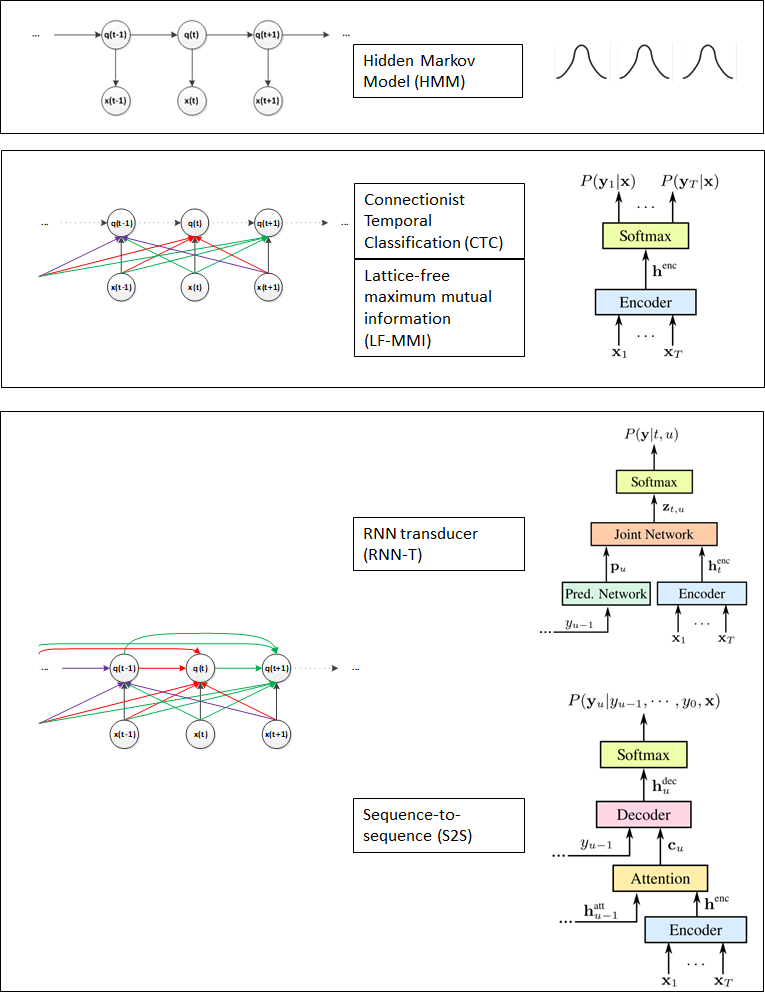
\includegraphics[clip=true, width=0.7\textwidth]{figure/e2e.png}
%    \bicaption[fig:e2e]{}{传统系统与端到端系统比较}{Fig}{Comparison of Various End-to-end Models}
%\end{figure}

\subsection{基于CTC的序列建模}
\label{Sec:sdm-sdt-intro}
%discriminate KW or discriminate KW \& filler, but filler is imperfect

{\em{鉴别式序列模型}} 是直接对序列后验概率进行估计的一类模型,如公式 (\ref{equ:ctc-model})所示,符合语音识别任务对序列后验概率$p(\mathbf{L}|\mathbf{O})$建模的需求。
连接时序分类模型 (CTC) 是一个典型的例子~\cite{graves2006connectionist,huang2018ctc},其目标函数为,
\begin{equation}
\label{equ:ctc-formu}
\begin{split}
P(\mathbf{w}_u|\mathbf{O}_u)
= \sum_{\mathbf{L}\in\mathcal{L}(\mathbf{w}_u)} P(\mathbf{L}|\mathbf{O}_u)P(\mathbf{w}_u|\mathbf{L})
\end{split}
\end{equation}
公式中 $\mathbf{L}$ 是CTC模型的标签序列,比如半词或者音素序列等, $\mathcal{L}$定义了从词序列 $\mathbf{w}$ 到它的标签序列 $\mathbf{L}$ 的映射。
语音识别中,CTC通常被用来建模半词或者音素序列等。
在~\cite{fernandez2007application}中, CTC被应用到KWS中,
其输出也可以被定义为所有可能的关键词序列 $\mathbf{w}$的后验概率。
在语音识别中,$P(\mathbf{w}_u|\mathbf{L})$ 由语言模型和词典给出。
在声学KWS中,没有引入语言模型,$P(\mathbf{w}_u|\mathbf{L})$ 是一个确定性的由词典到关键词序列的映射。
$P(\mathbf{L}|\mathbf{O}_u)$ 可以进一步映射到CTC模型的标签序列,并分解到每一帧,如公式 (\ref{equ:ctc-model})所示。
注意到一个额外的$\tt blank$ 单元被引入到逐帧的公式 (\ref{equ:ctc-model})中以建模语音信号的混淆区段。

对于传统DNN-HMM混合模型而言,我们通常选取帧层面的交叉熵函数作为代价函数对DNN模型进行更新,这个过程中预先需要由GMM模型提供训练语料的帧层面的对齐。连接时序分类模型(Connectionist Temporal Classification, CTC)提出自动学习输入帧特征序列与其对应标签序列之间的对齐关系。
其准则定义为所有可能的CTC标签序列的概率求和,作为最终的优化方向。

我们可以预先定义训练集的标签序列包含K个不同标签,这其中还包含意味着无发射标签的空符号标签$\tt blank$建模单元。我们定义输入帧特征序列以及相对应的标签序列。这样我们就可以通过在给定输入序列的条件下最大化标签序列的对数似然比,对预测模型进行更新。

然而由于标签并不是对齐到帧层面的,因此我们无法直接计算该似然比。为了建立前端预测模型输出与标签序列之间联系,
CTC模型被定义为标注序列在给定特征序列后的后验概率 $P(\mathbf{L}|\mathbf{O})$。
CTC引入上述 $\tt blank$ 状态来对标签之间的混淆区段进行建模。具体来说,模型在标注$l_{i-1}$ 和 $l_{i}$之间,通常预测出 $ \tt blank$ 标注。

\begin{equation}
\label{equ:ctc-model}
\begin{split}
P(\mathbf{L}|\mathbf{O})=\sum_{\mathbf{q}\in\mathcal{B}(\mathbf{L})}P(\mathbf{q}|\mathbf{O}) =\sum_{\mathbf{q}}\prod_{t=1}^{T} p(q_t|\mathbf{O})
\end{split}
\end{equation}
公式中 $\mathcal{B}$ 是一个一对多的映射函数~\footnote{在最早文献~\cite{graves2006connectionist}中使用的公式定义为一个多对一映射函数,同时使用它的反函数来定义 $\mathcal{B}^{-1}(\cdot)$ 表示CTC模型中的映射。这里我们修改为一个一对多映射函数,使公式与HMM中的定义更加一致。}:
\begin{equation}
\label{equ:ctc-b}
\begin{split}
\mathcal{B}:\mathbb{L}   \mapsto  \mathbb{L} \cup \{\tt blank\}
\end{split}
\end{equation}
$\mathcal{B}$ 决定了标签序列 $\mathbf{L}$ 和它相应由建模单元所组成的模型状态序列$\mathbf{q}$。 这一映射做法是在每个组成 $\mathbf{L}$ 的$l$的标签中,插入一个可选并且可重复的 $ \tt blank$ 标签。 $P(q_t|\mathbf{O})$是由深度学习模型直接根据给定的特征序列$\mathbf{O}$来估计得出的, 比如使用LSTM~\cite{hochreiter1997long}。 

\subsection{基于序列到序列模型的序列建模}
\label{chap:intro2-e2e-s2s}

另一类鉴别式序列模型称为序列到序列模型。下文讨论将以基于注意力机制的序列到序列模型(encoder-decoder模型)~\cite{chan2016end}为主进行介绍,该类模型也是当前主要研究热点。
该模型预测了在直接给定特征序列$\mathbf{O}$下的标签序列和之前已经预测出的标签历史序列$\mathbf{L}_{1:i-1}$后验概率。
\begin{equation}
\label{equ:enc-dec}
\begin{split}
P(\mathbf{L}|\mathbf{O})=\prod_i P(l_{i}|\mathbf{O},\mathbf{L}_{1:i-1})
\end{split}
\end{equation}
%An attention mechanism weights  hidden vectors of the audio feature sequence to pick the most related hidden vectors for prediction at every step of the output sequence.
\begin{equation}
%\vspace{-0.6em}
\label{equ:enc-dec-hid}
\begin{split}
\mathbf{H}&=\text{Encoder}(\mathbf{O})\\
\end{split}
\vspace{-0.3em}  
\end{equation}
\begin{equation}
\label{equ:enc-dec-dec}
P(l_{i}|\mathbf{O},\mathbf{L}_{1:i-1})=\text{AttentionDecoder}(\mathbf{H}, s_{i-1})
\end{equation}
在公式中, $\mathbf{H}$表示编码器(encoder)网络的隐层状态。$\mathbf{s_{i-1}}$表示解码器(decoder)的上一输出相应隐层状态。$\text{Encoder}(\cdot)$ 通常是一个单向或者多向的LSTM网络,同时 $\text{AttentionDecoder}(\cdot)$ 通常是一个单向LSTM网络。 %\addcomment{this notation is not clear, does $\mathbf{x}$ mean all features in th sequence? why subscript for time in $\mathbf{l}$ but superscript for $\mathbf{s}$ }

与传统混合系统~\cite{hinton2012deep}相比,该模型所使用的$\text{AttentionDecoder}(\cdot)$隐含地建模了语言模型信息,并将其与 $\text{Encoder}$所组成的声学模型进行联合训练。
%
%In the inference stage, AttentionDecoder uses hypotheses from previous steps and weighted average of encoder outputs to predict the next label. 
%
%Beam search is always applied to constrain the search space.
这种建模方式的优势包括:基于深度学习的历史建模,更强的序列建模能力,以及更好的系统联合训练。除此之外,得益于该模型融合了语音识别的所有知识源,由此模型训练和推理搜索的系统设计都将非常简洁。
但是由于该模型中的声学模型和语言模型进行了紧密的联合训练,这种系统并不容易被自适应到新的领域或者上下文环境中。与之相反,传统系统则可以通过直接修改语言模型而进行领域自适应~\cite{mcgraw2016personalized}。这是该模型的一个重要劣势,也是目前的研究热点之一~\cite{zhc00-chen-icassp19}。 

本论文主要关注可以进行帧级别分解的GSM及DSM模型,对于不进行显示帧分解的模型,只做部分涉及(第\ref{chap:lsd-e2e}章节)。

\section{语言识别中的端到端模型}
\label{chap:intro2-e2e}

第\ref{chap:intro2-dl-asr}章节介绍的传统DNN-HMM模型核心在于将整体语音识别系统依据人类语言的先验知识进行模块化(modularization),而后分部分建模,再使用第\ref{Sec:seq-tr-review}章节中的序列鉴别性训练技术进行联合调优。这样的系统普遍存在两部分潜在缺点:
\begin{itemize}
    \item 模块化限制了序列建模能力。模块化依据人类语言学知识来进行建模步骤的划分,但往往这些先验知识并不一定反应真实的自然语言现象。而模块化通常假设各模块之间是条件独立的(比如语言模型只建模词语之间的概率,而与声学特征无关),那么错误的条件独立假设将会限制最终系统的性能。这些条件独立假设通常出现在人类语言的不同粒度上(比如音素、字词),因此上述性能的限制就具体体现在序列建模能力上。
    \item 模块化使得系统构建步骤复杂。如第\ref{chap:intro-asr}章节所述,传统系统搭建步骤复杂,还需要大量人类数据科学家进行模型超参数调优。语音识别的广泛推广,使得对大量语言和大量工作场景的支持成为了迫切的需求,这就对系统搭建难度和速度提出了新的要求。同时语言学研究尚未深入涉及人类的大量语言,而DNN-HMM这类模块化系统较难在语言学知识缺失(比如音素集合缺失)的情况下被搭建。
\end{itemize}

\begin{figure}[!htp]
  \centering
    \captionstyle{\centering}
    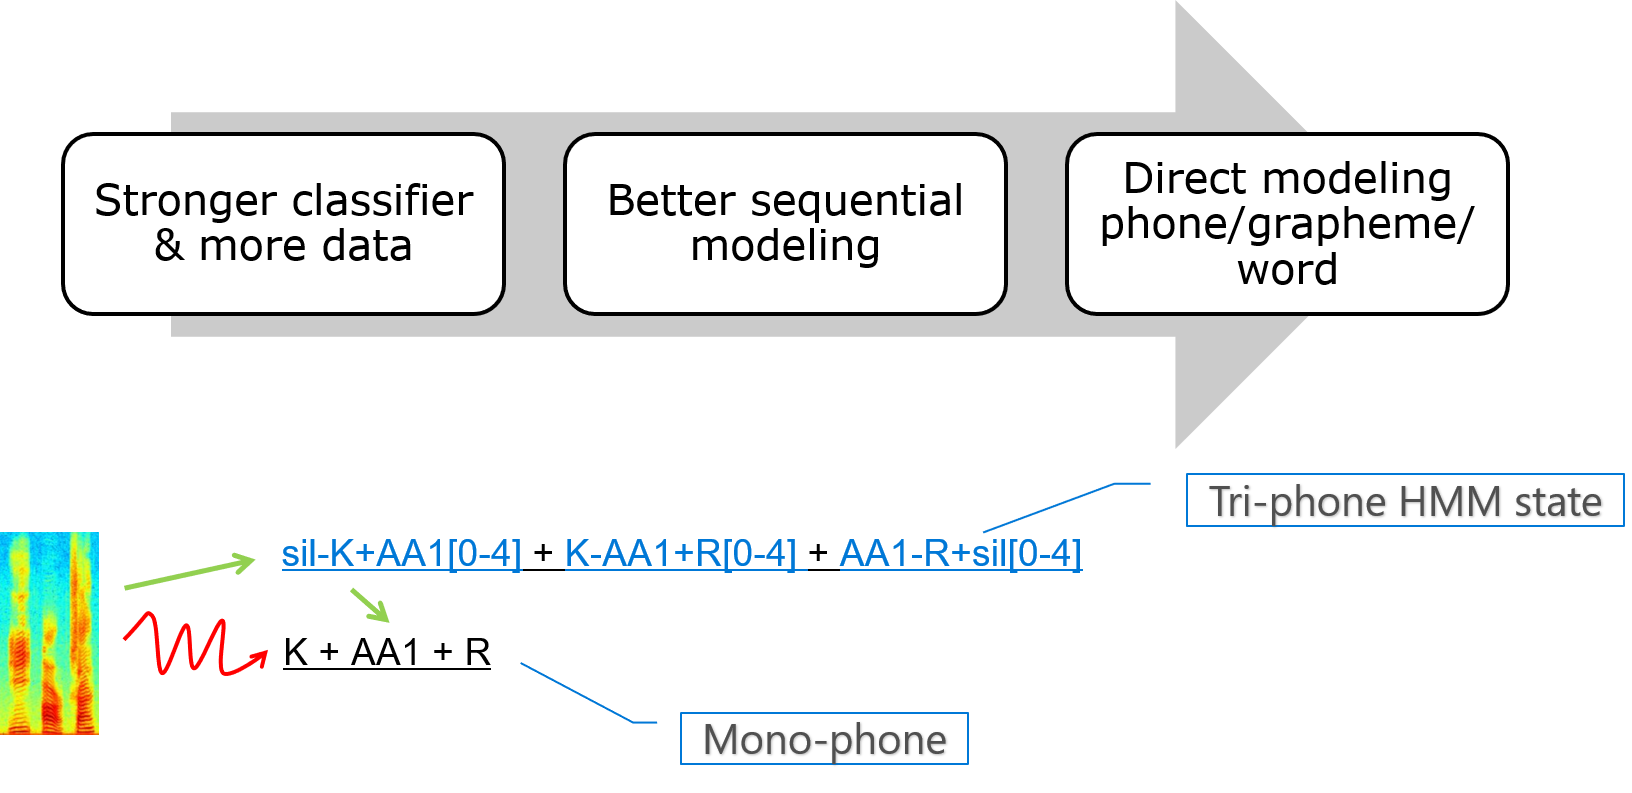
\includegraphics[clip=true, width=0.7\textwidth]{figure/e2e-idea.png}
    \bicaption[fig:e2e-idea]{}{端到端系统举例}{Fig}{Motivation and Example of End-to-end Modeling}
\end{figure}


得益于标注数据的增多和算力改善,深度学习模型取得了更强的分类能力。由此人们开始考虑直接使用深度序列模型对序列进行直接建模,以取得更好序列建模能力。我们称这种“直接建模”的发展趋势为“端到端”。如图~\ref{fig:e2e-idea}所示,原来传统系统中的音素声学建模可以直接被深度模型所取代,由此直接对词语或单字进行建模。
% TODO: mod fig
值得注意的是,根据上一章节中的分类,这类模型绝大部分为{\em 鉴别式序列模型}, 由 $P(\mathbf{L}|\mathbf{O})$进行定义,表示给定特征序列$\mathbf{O}$直接建模输出序列 $\mathbf{L}$的后验概率。
这类鉴别式序列模型包括CTC,序列到序列模型等。

在上述模型中,所建模的输出序列$\mathbf{L}$(模型输出粒度)可以是词语(word)或单字(grapheme or character),字母(letter)。
在有些研究中使用byte-pair encoding (BPE),因为其映射到词语的方式比较直接,也可以认为是一种端到端的建模系统;后文中我们将以由声学特征直接建模词语序列(Acoustic-to-word, A2W)的方式为主进行讨论。




\section{本章小结}
\label{chap:intro-sum}

在这章中我们首先简要介绍了语音信号的识别的基本内容,包括特征提取,声学模型,语言模型和Viterbi解码等内容。
%
紧接着我们回顾了语音识别中最常用神经网络结构,主要包括深度神经网络、卷积神经网络、循环神经网络。接着探讨了神经网络的训练方法,包括训练准则、反向传播算法以及一些实际优化细节。随后回顾了深度神经网络-隐马尔科夫模型混合系统,这是目前语音识别领域最有效的将DNN与HMM结合的办法。
接着引出了目前研究的热点,即端到端语音识别系统。我们系统介绍了端到端建模各个变种,它们的特点及优势,为之后几章改进和推理搜索框架研究进行了铺垫。